\setchapterstyle{kao}
\setchapterpreamble[u]{\margintoc}
\chapter{Neutrino Oscillations}
\labch{massoscillations}

As outlined in \refsec{neutrino-masses}, flavor eigenstates of neutrinos are not identical to their mass eigenstates. After they acquire their mass via electroweak symmetry breaking, the mass and flavor eigenstates mix among each other via the PNMS matrix $U$ that, in the case of pure Dirac masses, is a $3\times3$ unitary matrix. Thus, the eigenstate for a neutrino flavor $\alpha$ can be described as a superposition of mass eigenstates as
\begin{equation}
    \ket{\nu_\alpha} = \sum_k U^*_{\alpha k}\ket{\nu_k}\;.\label{eq:flavor-state-def}
\end{equation}
This has profound consequences for the propagation of neutrinos, because the wavepackets of the different mass eigenstates do not travel at exactly the same speed. The lighter states are faster than the heavier ones, which causes the waves to interfere with one another constructively or destructively as long as the wave packets still overlap. This chapter describes neutrino oscillations in vacuum and in matter under the simplifying assumption that the mass eigenstates are ideal plane waves. The fact that they are actually wave packets with an uncertain energy and a finite extent leads to decoherence for very large propagation distances or mass differences. While this is irrelevant for the standard three-flavor oscillation result of this work, it does put an upper limit on the mass splitting for which the sterile oscillation result is valid. This will be described briefly at the end of this chapter.

\section{Neutrino Oscillations in Vacuum}

The simplest case to describe is that of neutrino oscillations in vacuum. The propagation of these states is governed by the Schrödinger equation
\begin{equation}
    i \dv{t} \ket{\nu_k(t)} = \mathcal{H} \ket{\nu_k(t)}
\end{equation}
with the plane-wave solution
\begin{equation}
    \ket{\nu_k(t)} = e^{-iE_k t} \ket{\nu_k}\;.\label{eq:schrodinger-eq}
\end{equation}
Substituting the flavor eigenstate from \refeq{flavor-state-def} into \refeq{schrodinger-eq} using the relation $U^\dag U=\mathbb{1}$, the propagation becomes
\begin{equation}
    \ket{\nu_\alpha(t)} = \sum_{\beta=e,\mu,\tau} \left(\sum_k U^*_{\alpha k} e^{-iE_k t}  U^*_{\beta k}\right) \ket{\nu_\beta}\;.\label{eq:flav-evolution}
\end{equation}
This leads directly to the expression for the probability to measure one flavor after a given time
\begin{equation}
    P_{\nu_\alpha \rightarrow \nu_\beta} = \abs{\braket{\nu_\beta}{\nu_\alpha(t)}}^2
    = \sum_{k,j}U^*_{\alpha k}U_{\beta k}U_{\alpha j}U_{\beta j}^* e^{-i(E_k - E_j)t}\;.
\end{equation}
If we assume that all mass eigenstates have the same momentum\sidenote[][*1]{The equal momentum assumption is not exactly realistic, but more detailed derivations can show that deviations from it cause no observable effect. See also chapter 8.1.2 in \cite{giunti-kim-neutrino}.} and that they are highly relativistic, we can approximately express the energy in terms of the mass of each state
\begin{equation}
    E_k = \sqrt{\vec{p}^2 + m_k^2} \simeq E + \frac{m_k^2}{2E}
\end{equation}
and write the transition probability in terms of the energy and the differences of squared masses between the mass eigenstates
\begin{equation}
    \Delta m_{kj}^2 \equiv m_k^2 - m_j^2
\end{equation}
and the travelled distance, $L$, as
\begin{equation}
    P_{\nu_\alpha \rightarrow \nu_\beta}(L,E) = \sum_{k,j}U^*_{\alpha k}U_{\beta k}U_{\alpha j}U_{\beta j}^* \exp(-i\frac{\Delta m_{kj}^2 L}{2E})\;.\label{eq:vac-oscprob}
\end{equation}
This state evolution can also be expressed with the effective Hamiltonian
\begin{equation}
    \mathcal{H}_\mathrm{eff} = \frac{1}{2E}U\mathrm{diag}(0,\Delta m_{21}^2, \Delta m_{31}^2)U^\dag
\end{equation}
and one can define the characteristic distance for oscillations between mass eigenstates $k$ and $j$ at which the oscillation amplitude is maximal as
\begin{equation}
    L_{kj}^\mathrm{osc} = \frac{4\pi E}{\Delta m_{kj}^2}\;.
\end{equation}
Antineutrino flavor eigenstates are superpositions of corresponding antineutrino mass eigenstates, and they are related by the complex-conjugated PNMS matrix such that
\begin{equation}
    \ket{\bar{\nu}_\alpha} = \sum_k U_{\alpha k}\ket{\bar{\nu}_k}\;.\label{eq:flavor-state-def-antinu}\;.
\end{equation}
This leads to the same expression for their oscillation probability as in \refeq{vac-oscprob}, except that all elements of $U$ are complex-conjugated.

\subsection{Two-neutrino mixing}
\labsubsec{two-neutrino-mixing}
Neutrino oscillation experiments are typically limited to a certain oscillation length and energy range that they can probe. Because the two mass splittings between the three known neutrino flavors are two orders of magnitude apart ($\order{\SI{e-5}{eV^2}}$ for $\Delta m^2_{21}$ vs. $\order{\SI{e-3}{eV^2}}$ for $\Delta m^2_{32}$), each experiment is in practice much more sensitive to one of them than to the other. Therefore, a good first approximation to calculate neutrino oscillation probabilities is to only consider two flavor and two mass eigenstates with a mass splitting of $\Delta m^2 \equiv m_2^2 - m_1^2$ that mix via the rotation matrix
\begin{equation}
    U =
    \begin{pmatrix}
        \cos \vartheta & \sin \vartheta \\
        -\sin \vartheta & \cos \vartheta
    \end{pmatrix}\;,\label{eq:two-flav-pnms}
\end{equation}
where the angle $\vartheta$ is the \emph{mixing angle} between the two mass eigenstates. The transition probability from flavor $\alpha$ to $\beta$ with $\alpha \neq \beta$ can be quickly derived from the general \refeq{vac-oscprob} to be
\begin{equation}
    P_{\nu_\alpha \rightarrow \nu_\beta} = \sin^2 2\vartheta \sin[2](\frac{\Delta m^2L}{4E})\qc\alpha \neq \beta\;.
\end{equation}
Conversely, the probability that an initial flavor $\alpha$ is still being measured as $\alpha$ after a given propagation distance, also referred to as the \emph{survival probability}, is
\begin{equation}
    P_{\nu_\alpha \rightarrow \nu_\alpha} = 1 - \sin^2 2\vartheta \sin[2](\frac{\Delta m^2L}{4E})\;.
\end{equation}

\section{Oscillations in matter}
The oscillation probabilities derived in the previous sections for the vacuum are altered significantly when neutrinos pass through large amounts of matter, as it is the case for neutrinos originating in the atmosphere of the Earth that pass through its dense core to be detected at the South Pole. The effect can be described as a continuous potential that is added to the Hamiltonian in the flavor basis that corresponds to the isoscalar (nulcei) targets and electrons inside the Earth. The detailed derivation of this matter potential can be found in \sidecite{matter-potentials} and we will only briefly outline the process here. We will also describe how the matter potential leads to an enhancement of effective mixing between flavors in the simplified picture of two flavors and a constant matter density.

\subsection{Effective potentials}
At energies relevant to this work\sidenote{Incoherent scattering becomes only important at energies above $\order{\SI{e5}{GeV}}$.}, neutrinos are mostly affected by coherent forward scattering processes, that is, scattering with a very small momentum transfer. The Feynman diagrams of the relevant processes are shown in \reffig{coh-scatter-feynman}. All neutrino flavors can interact with electrons and nuclei via the neutral-current (NC) interaction, while only electron-neutrinos can also undergo charged-current (CC) scattering off of electrons.
\begin{figure}
\def\flen{2}
\def\boslen{1.5}
\def\fang{25}
\begin{subfigure}[t]{0.49\linewidth}
\begin{tikzpicture}
    \begin{feynman}
        \vertex (v1) [dot] at (0, \boslen) {};
        \vertex (i1) at ($(v1) + (180-\fang:\flen)$) {$\nu_e$};
        \vertex (f1) at ($(v1) + (\fang:\flen)$) {$e^-$};

        \vertex [dot] (v2) at (0, 0) {};
        \vertex (i2) at ($(v2) + (\fang-180:\flen)$) {$e^-$};
        \vertex (f2) at ($(v2) + (-\fang:\flen)$) {$\nu_e$};

        \diagram*{
            (i1) -- [fermion] (v1) -- [fermion] (f1),
            (i2) -- [fermion] (v2) -- [fermion] (f2),
            (v1) -- [boson, edge label=$W^+$] (v2)
        };
    \end{feynman}
\end{tikzpicture}
\caption{Charged-current\label{fig:coh-scatter-cc}}
\end{subfigure}
\begin{subfigure}[t]{0.49\linewidth}
\begin{tikzpicture}
    \begin{feynman}
        \vertex (v1) [dot] at (0, \boslen) {};
        \vertex (i1) at ($(v1) + (180-\fang:\flen)$) {$\nu_e,\nu_\mu,\nu_\tau$};
        \vertex (f1) at ($(v1) + (\fang:\flen)$) {$\nu_e,\nu_\mu,\nu_\tau$};

        \vertex [dot] (v2) at (0, 0) {};
        \vertex (i2) at ($(v2) + (\fang-180:\flen)$) {$e^-, p, n$};
        \vertex (f2) at ($(v2) + (-\fang:\flen)$) {$e^-, p, n$};

        \diagram*{
            (i1) -- [fermion] (v1) -- [fermion] (f1),
            (i2) -- [fermion] (v2) -- [fermion] (f2),
            (v1) -- [boson, edge label=$Z^0$] (v2)
        };
    \end{feynman}
\end{tikzpicture}
\caption{Neutral-current}
\end{subfigure}
\caption{Feynman diagrams of the coherent forward scattering processes for neutrinos travelling through Earth.\label{fig:coh-scatter-feynman}}
\end{figure}
When the exchanged momentum is small, then the propagator in each Feynman diagram can be contracted into a 4-point Fermi interaction with the coupling constant $G_F$. The effective CC Hamiltonian for the diagram in \reffig{coh-scatter-cc} (after a Fierz transformation) becomes
\begin{equation}
    \mathcal{H}_\mathrm{eff}^{CC}(x) = \frac{G_F}{\sqrt{2}}
    [\bar{\nu}_e(x)\gamma^\rho(1 - \gamma^5)\nu_e(x)]
    [\bar{e}(x)\gamma_\rho(1 - \gamma^5)e(x)]\;.\label{eq:h-eff-cc}
\end{equation}
This Hamiltonian is then averaged over the momenta and helicities of a constant density of electrons with the result
\begin{equation}
    \overline{\mathcal{H}_\mathrm{eff}^{CC}}(x) = V_{CC} \bar{\nu}_{e,L}(x)\gamma^0\nu_{e,L}(x)\;,
\end{equation}
where $V_{CC}$ is the charged-current potential
\begin{equation}
    V_{CC} = \sqrt{2}G_F N_e
\end{equation}
with the electron number density $N_e$. The derivation of the NC potential follows in similar steps with the addition of a different coupling constant for electrons, protons, and electrons. For electrically neutral media, the potentials for protons and electrons exactly cancel and the only remaining NC potential comes from the neutron density, $N_n$, and is given by
\begin{equation}
    V_{NC} = -\frac{1}{2}\sqrt{2}G_F N_n\;.
\end{equation}
With the addition of these potentials, the effective Hamiltonian governing the evolution of flavor states for neutrinos propagating in matter is
\begin{equation}
\mathcal{H}_\mathrm{eff}(E,x) = \mathcal{H}_0(E)  + \mathcal{H}_{1}(E,x)\;,
\end{equation}
with
\begin{subequations}
\label{eq:hamiltonian}
\begin{align}
\mathcal{H}_0 (E) &= \frac{1}{2E} U
\mqty(\dmat{0 , \Delta m^2_{21}, \Delta m^2_{31}})
U^\dag \label{eq:h0-flav-basis}\;,\\
\mathcal{H}_1 (E,x) &= \frac{\sqrt{2}}{2} G_F
\mqty(\dmat{2N_e(x) - N_n(x), -N_n(x), -N_n(x)})
\;.\label{eq:hi-flav-basis}
\end{align}
\end{subequations}
The NC potential in \refeq{hi-flav-basis} can be neglected in the case of three-flavor oscillations, because a diagonal contribution to the Hamiltonian merely adds an unobservable phase shift that affects all flavors equally. However, if sterile Majorana  mass eigenstates are added, their corresponding matter potentials are zero and they only add their respective mass splitting to \refeq{h0-flav-basis}. In that case, the state evolution has to be described using both CC and NC potentials.

\subsection{The MSW Effect}
An interesting consequence of matter potentials is that they can greatly enhance the mixing amplitude between flavors over that of vacuum oscillations. The effect is straight forward to illustrate for the case of two-flavor oscillations, where one flavor feels a potential, $V$, and the other does not. With the mass-splitting $\Delta m^2 \equiv m_2^2 - m_1^2$ and $2\times2$ mixing matrix from \refeq{two-flav-pnms}, the effective Hamiltonian for this scenario is
\begin{equation}
\begin{aligned}
    \mathcal{H}  &= \frac{1}{4E}\left(
        U\mqty(\dmat{0, \Delta m^2})U^\dag + \mqty(\dmat{A_\mathrm{CC}, 0})
    \right)\\
    &= \frac{1}{4E} \mqty(
        -\Delta m^2 \cos 2\vartheta + A_\mathrm{CC} & \Delta m^2 \sin 2\vartheta \\
        \Delta m^2 \sin 2\vartheta & \Delta m^2 \cos 2\vartheta - A_\mathrm{CC}
    )\;,
\end{aligned}
\end{equation}
where we have subtracted $\frac{1}{4E}(\Delta m^2 + A_\mathrm{CC})$ from the diagonal in the second line with $A_\mathrm{CC} = 2E V$. This Hamiltonian can be diagonalized by another 2D rotation matrix $U_M$, with mixing angle $\vartheta_M$, such that
\begin{equation}
    U_M^T\mathcal{H}U_M = \mathcal{H}_M = \frac{1}{4E}\mqty(\dmat{-\Delta m^2_M, \Delta m^2_M})
\end{equation}
is diagonal. The diagonalization is achieved under the condition
\begin{equation}
    \tan 2\vartheta_M = \frac{\tan 2\vartheta}{1 - \frac{A_\mathrm{CC}}{\Delta m^2 \cos 2\vartheta}}\;,\label{eq:msw-condition}
\end{equation}
leading to a new effective mass splitting in matter,
\begin{equation}
    \Delta m^2_M = \sqrt{(\Delta m^2 \cos 2\vartheta - A_\mathrm{CC})^2 + (\Delta m^2\sin 2\vartheta)^2}\;.
\end{equation}
As a consequence of the condition in \refeq{msw-condition}, the effective mixing angle in matter can become maximal under the condition that
\begin{equation}
    V = \frac{\Delta m^2 \cos 2\vartheta}{2E_\mathrm{res}}\label{eq:msw-pot}
\end{equation}
with the resonance energy $E_\mathrm{res}$.
This enhancement of mixing between flavors due to the presence of a matter potential is known as the \emph{MSW effect}, named after Mikheev, Smirnov, and Wolfenstein. It is primarily responsible for the fact that there is a sizable disappearance of electron neutrinos from the sun despite the fact that the relevant vacuum mixing angle is rather small.
The potential for isoscalar targets is
\begin{equation}
    V = \sqrt{2}G_F N_e \approx Y_e \times \qty[\frac{\rho}{\si{\gram\per\cm\cubed}}] \times \SI{7.63e-14}{\electronvolt}\;,\label{eq:pot-isoscalar}
\end{equation}
where $Y_e = N_e / (N_p + N_n)$ is the electron fraction in the medium and is usually close to $\frac{1}{2}$.
%which corresponds to an electron number density of
%\begin{equation}
%    N_e = \frac{\Delta m^2 \cos 2\vartheta}{2\sqrt{2}E G_F}\;.\label{eq:msw-electron-density}
%\end{equation}
%Taking the density of the core of the Earth, $\rho_\mathrm{core} \approx \SI{13}{\gram\per\cubic\centi\meter}$, we find
%\begin{equation}
%    N_{e,\mathrm{core}} \approx \SI{13}{\gram\per\cubic\centi\meter}\times \frac{1}{2} \times \SI{1}{\mole\per\gram} \times N_A \approx \SI{4e24}{\per\cubic\centi\meter}\;,
%\end{equation}
%we find
We can find the resonant energy where the MSW resonance occurs for a given matter density by combining \cref{eq:msw-pot,eq:pot-isoscalar} into
\begin{equation}
    E_\mathrm{res} = \frac{\Delta m^2 \cos 2\vartheta}{2V} \approx \frac{(\Delta m^2\si{\per\electronvolt\squared}) \cos 2\vartheta}{Y_e \qty[\frac{\rho}{\si{\gram\per\cm\cubed}}]}\times\SI{6.6e12}{\electronvolt}\;.
\end{equation}
For three-flavor oscillations observed experimentally, the MSW resonance can enhance mixing due to the relatively small mixing angle $\theta_{13}=\SI{8.6+-0.13}{\degree}$\cite{pdg}.  This occurs at $\approx \SI{7}{\giga\electronvolt}$ for muon neutrinos travelling through the mantle of the Earth, where the density is $\rho_\mathrm{mantle}\approx\SI{4.5}{\gram\per\cubic\centi\meter}$ and where the observed oscillations are due to the larger mass splitting $\Delta m^2_{32}\approx \SI{2.5e-3}{\electronvolt\squared}$.
For hypothetical sterile neutrinos with a mass splitting of $\order{\SI{1}{\electronvolt}}$ passing through the core of the Earth with $\rho\approx\SI{13}{\gram\per\cubic\centi\meter}$ and $Y_e\approx\frac{1}{2}$, this gives a resonant energy of close to \SI{1}{\tera\electronvolt} assuming a small mixing angle between active and sterile flavors. This effect has been used in previous IceCube studies\cite{MEOWS} to search for traces of sterile neutrinos using TeV~scale atmospheric neutrinos, but it is not relevant to the analysis presented in this work.

\subsection{Parametric resonance}
Another way in which the presence of matter potentials can enhance neutrino oscillation amplitudes is via parametric resonance. This resonance occurs when the matter potential changes abruptly at just the right frequency to create a situation that is analogous to constructive interference, even if the density is far from the MSW resonance condition. The reason why this can happen is that the quantum state of the neutrino receives a phase shift at every interface between regions of different densities. If such an interface is located at the oscillation maximum and the difference in densities has the right magnitude, the phase is reset to zero and and the flavor transition probability will increase again in the next region, instead of returning to zero. This situation can arise in particular at the transition points between the mantle and the core when neutrinos pass through the Earth as shown in \reffig{parametric-resonance}. The black solid line shows the matter potential that is used to approximate the matter potential for the oscillation calculation. At each interface (dashed lines), the phase shift causes the oscillation pattern to begin at the rising flank again. After the neutrino propagates through the Earth, the oscillation probability has increased to close to one.
\begin{figure}
    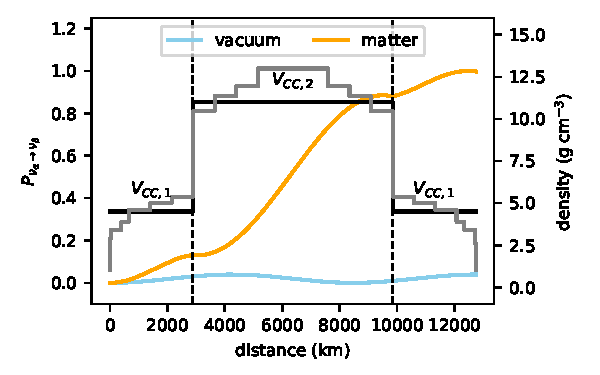
\includegraphics[width=4in]{figures/theory/parametric_resonance.pdf}
    \caption{Parametric resonance for a simplified mantle-core-mantle propagation with two flavors. The assumed mass-splitting is $\Delta m^2=\SI{2.5e-3}{eV^2}$, the mixing angle is $\theta=\arcsin(0.1)$, and the energy is \SI{3.4}{GeV}. The matter potential used for the calculation is shown in black. The gray line in the background shows the density profile of Earth in the 12-layer PREM model.\label{fig:parametric-resonance}}
\end{figure}
The condition for maximum parametric resonance is delicately dependent on the energy, mass splitting, mixing angle, and the parameters of the matter potential and are derived in more detail in \cite{Akhmedov:1999ty}. In atmospheric neutrino oscillations, parametric enhancement of the $\nu_\mu\rightarrow\nu_e$ oscillation channel is responsible for the distortions of the oscillation pattern at a few GeV.


\subsection{Neutrino Mass Ordering}
In vacuum, neutrino oscillations are only sensitive to the absolute differences between (squared) neutrino masses, not their sign. As a result, there are two degenerate possibilities to arrange the mass eigenstates that produce the same vacuum oscillation effect. The case where $m^2_1 < m^2_2 < m^2_3$ is referred to as \emph{normal ordering}. In this case, the value of the mass splitting $\Delta m^2_{ij}$ is always positive for $i>j$. In the case of \emph{inverted ordering}, we have $m^2_3 < m^2_1 < m^2_2$. In that case, the sign of $\Delta m^2_{32}$ is negative. While the ordering has no observable effect in vacuum, it does affect the propagation in the presence of matter effects. This can be seen readily in the MSW resonance condition in \refeq{msw-condition}, where the sign of $\Delta m^2$ enters in the denominator. The resonance condition for neutrinos can only be fulfilled if the sign of $\Delta m^2$ is the same as $\cos 2\theta$ for neutrinos, or if the signs of $\Delta m^2$ and $\cos 2\theta$ are different for antineutrinos. Therefore, the neutrino mass ordering can be determined experimentally by measuring the differences in matter effects between neutrinos and antineutrinos.

\section{Standard three-flavor oscillations}
The simplest extension to the Standard Model that explains the phenomenon of neutrino oscillations is that of three oscillating flavor eigenstates and three mass eigenstates that result from pure Dirac masses as described in \refsec{neutrino-masses}. In this picture, the mixing between mass eigenstates and is governed by the $3\times3$ PNMS matrix that is commonly parametrized by three mixing angles and one complex phase
\begin{equation}
\begin{aligned}
    U &=
    \begin{pmatrix}
    U_{e1}    & U_{e2}    & U_{e3}    \\
    U_{\mu1}  & U_{\mu2}  & U_{\mu3}  \\
    U_{\tau1} & U_{\tau2} & U_{\tau3} \\
    \end{pmatrix} \\
    &=
    \begin{pmatrix}
        c_{12} c_{13} & s_{12} c_{13} & s_{13}e^{-i\delta}       \\
        -s_{12}c_{23} - c_{12}s_{23}s_{13}e^{i\delta} & c_{12}c_{23}-s_{12}s_{23}s_{13}e^{i\delta} & s_{23}c_{13} \\
        s_{12}s_{23}-c_{12}c_{23}s_{13}e^{i\delta} & -c_{12}s_{23}-s_{12}c_{23}s_{13}e^{i\delta} & c_{23}c_{13}
    \end{pmatrix}\;,
\end{aligned}\label{eq:pnms-parametrization}
\end{equation}
where $s_{ij}$ and $c_{ij}$ are, respectively, the sine and cosine of the mixing angle $\theta_{ij}$. The complex phase $\delta$ leads to CP-violation of the oscillations. In addition, there are two mass splitting values between the three mass eigenstates, $\Delta m^2_{21}$ and $\Delta m^2_{31}$, that govern the frequency of the oscillations.
The most recent global best fit point\cite{Esteban:2020cvm} of the mixing angles and mass splittings under the assumption of normal neutrino mass ordering is shown in \reftab{global-bfp}. The table also lists the experimental channels that are primarily used to measure each parameter\todo{make table a bit nice, maybe include IO}.
\begin{table}
\caption{Best fit values of three-flavor oscillation parameters and the oscillation channel that is primarily involved in their measurement.\label{tab:global-bfp}}
\begin{tabular}{ccc}\toprule
    parameter & global fit & experimental channel \\ \midrule
    $\theta_{12}/^\circ$                    & $33.44^{+0.77}_{-0.74}$   & $\nu_e \rightarrow \nu_e$ (solar)\\
    $\frac{\Delta m^2_{21}}{\SI{e-5}{eV^2}}$& $7.42^{+0.21}_{-0.20}$    & $\bar{\nu}_e \rightarrow \bar{\nu}_e$ (reactor)\\
    $\theta_{23}/^\circ$                    & $49.2^{+1.0}_{-1.3} $     & $\nu_\mu \rightarrow \nu_\mu$  (atmospheric, accelerator)\\
    $\frac{\Delta m^2_{31}}{\SI{e-3}{eV^2}}$& $2.515^{+0.028}_{-0.028}$ & \\
    $\theta_{13}/^\circ$                    & $8.57^{+0.13}_{-0.12} $   & $\bar{\nu}_e \rightarrow \bar{\nu}_e$ (reactor)\\
    $\delta_\mathrm{CP}/^\circ$             & $194^{+52}_{-25}$         & $\nu_\mu \rightarrow \nu_e$ (accelerator)\\ \bottomrule
\end{tabular}
\end{table}

Different neutrino oscillation experiments probe different parts of the PNMS matrix and mass splitting. Broadly speaking, experiments can be divided into two categories by the mass-splitting that they can probe, which is determined by the oscillation length and energy spectrum of the experimental setup. The requirement to resolve oscillations is that the argument of the oscillation is $\Delta m^2 L/(2E) \sim \order{1}$. The larger of the two mass splittings is $\Delta m^2_{21} \sim \order{\SI{e-5}{eV^2}}$ and the smaller mass splitting is $\abs{\Delta m^2_{31}} \sim \order{\SI{e-3}{eV^2}}$. \reffig{oscillation-experiments-overview} gives an overview over different experiments, both operational and planned, with their respective energy ranges and baselines.
\begin{figure}
    \centering
    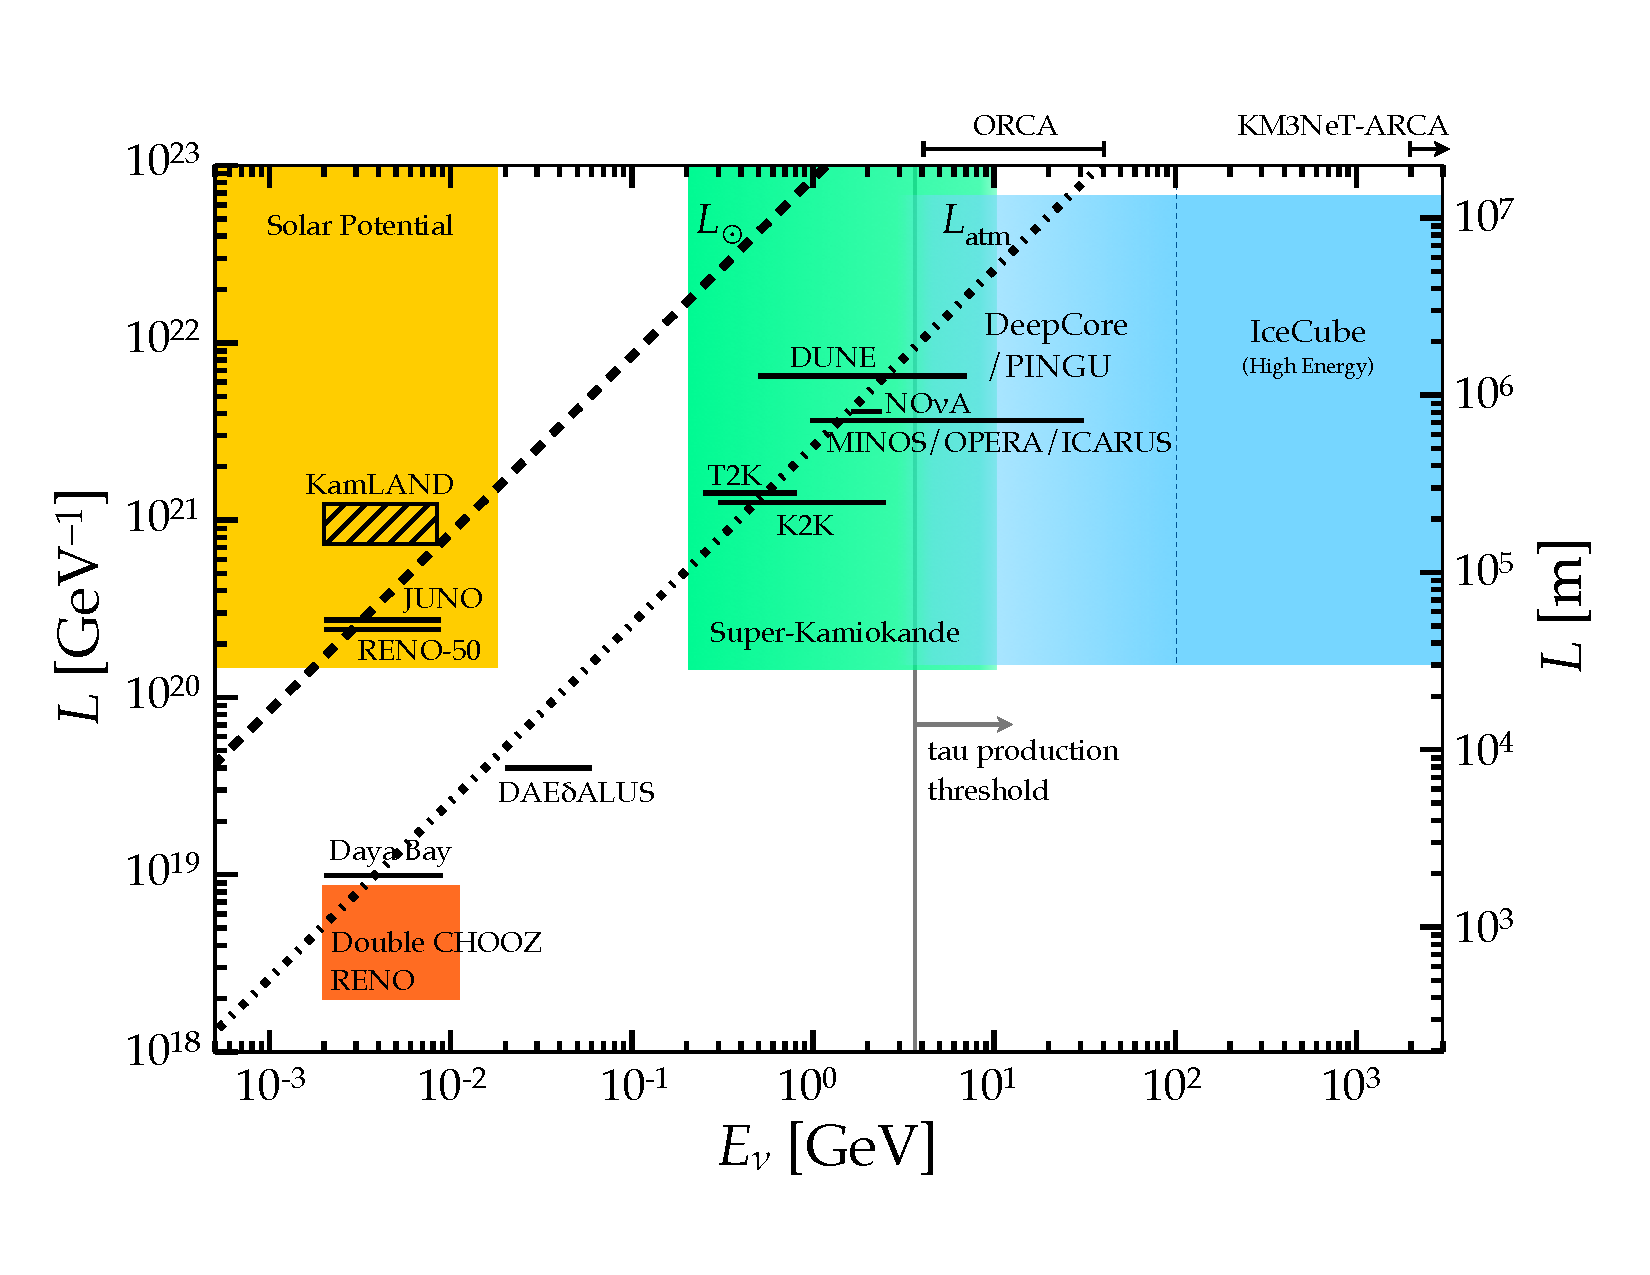
\includegraphics{figures/theory/LvsE.pdf}
    \caption{Energy ranges and baselines for a selection of neutrino oscillation experiments, operational or planned. Experiments on the line marked $L_{\odot}$ probe the solar mass splitting of $\order{\SI{e-5}{eV^2}}$, while those on the line marked $L_\mathrm{atm}$ measure oscillations at the atmospheric mass splitting of $\order{\SI{e-3}{eV^2}}$. The range of each experiment is shown either as a line for experiments with a fixed oscillation distance such as T2K or DUNE, or as a box for experiments with both a variable baseline and energy range such as IceCube. Figure taken from\cite{IceCube:2016xxt}.\label{fig:oscillation-experiments-overview}}
\end{figure}

\subsection{Solar neutrinos}
The mixing angles that parametrize the PNMS matrix and the mass splittings are typically associated with types of experiments that are most sensitive to them based on the oscillation channel that they observe. Since the angle $\theta_{13}$ is small, the PNMS matrix in \refeq{pnms-parametrization} can be decomposed to a first approximation into the upper left and lower right $2\times2$ blocks. The upper left block governs the transitions between $\nu_e$ and $\nu_\mu$ flavors with the mixing angle $\theta_{12}$ and the small mass splitting $\Delta m^2_{21}$. Such transitions are observed mainly by measurements of the neutrino flux originating from the Sun. For this reason, the mixing angle $\theta_{12}$ is also referred to as the ``solar angle`` and $\Delta m^2_{21}$ as the ``solar mass splitting``. Measurements of the solar neutrino flux are the oldest hints at neutrino oscillations and began at the end of the 1960s with the Homestake\cite{DAVIS199413} experiment. It used the inverse beta-decay process $^{37}\mathrm{Cl}+\nu_e \rightarrow e^- + ^{37}\mathrm{Ar}$ to capture neutrinos with an energy threshold of \SI{0.814}{MeV}. The observed neutrino flux was only about 30\% of the expectation, giving rise to the \emph{solar neutrino problem}. This problem was resolved in 2002, when observations at the Sudbury Neutrino Observatory (SNO) confirmed\cite{PhysRevLett.89.011301} that this deficit is due to a conversion of electron neutrinos into muon neutrinos, while the total neutrino flux, as measured by the rate of neutral-current interactions, stays constant. Terrestrially, these oscillations can only be observed using very low energy neutrinos from nuclear fission reactors at baselines of hundreds of kilometers. The only experiment of this kind that is currently operational is the KamLAND detector\cite{PhysRevLett.90.021802}.

\subsection{Reactor neutrinos}
The effect of the smaller mixing angle $\theta_{13}$ is in the sector of electron is that of a disappearance of electron neutrinos at short distances. Such measurements can be made using electron antineutrinos that are produced by fission reactors. Thus, the angle $\theta_{13}$ is also called the ``reactor`` angle. One experiment that is undertaking such measurements is the Daya Bay Reactor Neutrino Experiment\cite{DayaBay:2007fgu}. It consists of several detectors arranged around the reactor cores of the Daya Bay nuclear power plant that measure the electron antineutrino flux at different baselines. Comparative measurements between these detectors allows the mixing angle $\theta_{13}$ to be precisely determined while cancelling most of the systematic uncertainties of the experiment.

\subsection{Atmospheric Neutrino Oscillations}
\labsec{atmospheric-neutrino-oscillations}
The lower right block of the PNMS matrix controls transitions between $\nu_\mu$ and $\nu_\tau$ flavors with the mixing angle $\theta_{23}$ and large mass splitting $\Delta m^2_{32}$. These transitions are primarily observed by measuring the survival probability of muon neutrinos that are produced in the atmosphere of the Earth. Therefore, $\Delta m^2_{32}$ and $\theta_{23}$ are referred to as the ``atmospheric`` mass splitting and mixing angle, respectively. The first experiment that was able to measure the effect of atmospheric neutrino oscillations is the Super-Kamiokande experiment\cite{PhysRevLett.81.1562}, a Cherenkov neutrino detector located in the Kamioka mountains in Japan. The measurement presented in this work is also a measurement of atmospheric neutrino oscillations.

\subsubsection{Neutrino production in the atmosphere}
Neutrinos are produced in the atmosphere of the Earth when highly energetic cosmic radiation interacts with its upper layers. This cosmic radiation is composed of mostly fast protons and helium nuclei, and to a smaller fraction of other elements. The composition and spectrum of this radiation has been measured extensively by experiments conducted at high altitudes, such as in weather balloons, satellites, and on the International Space Station. The flux of cosmic rays as a function of energy per particle is shown in \reffig{cr-primary-flux}. From a few GeV to approximately \SI{100}{TeV}, it can be well approximated by a power spectrum with a spectral index of $\gamma \approx 2.7$.
\begin{figure}
    \centering
    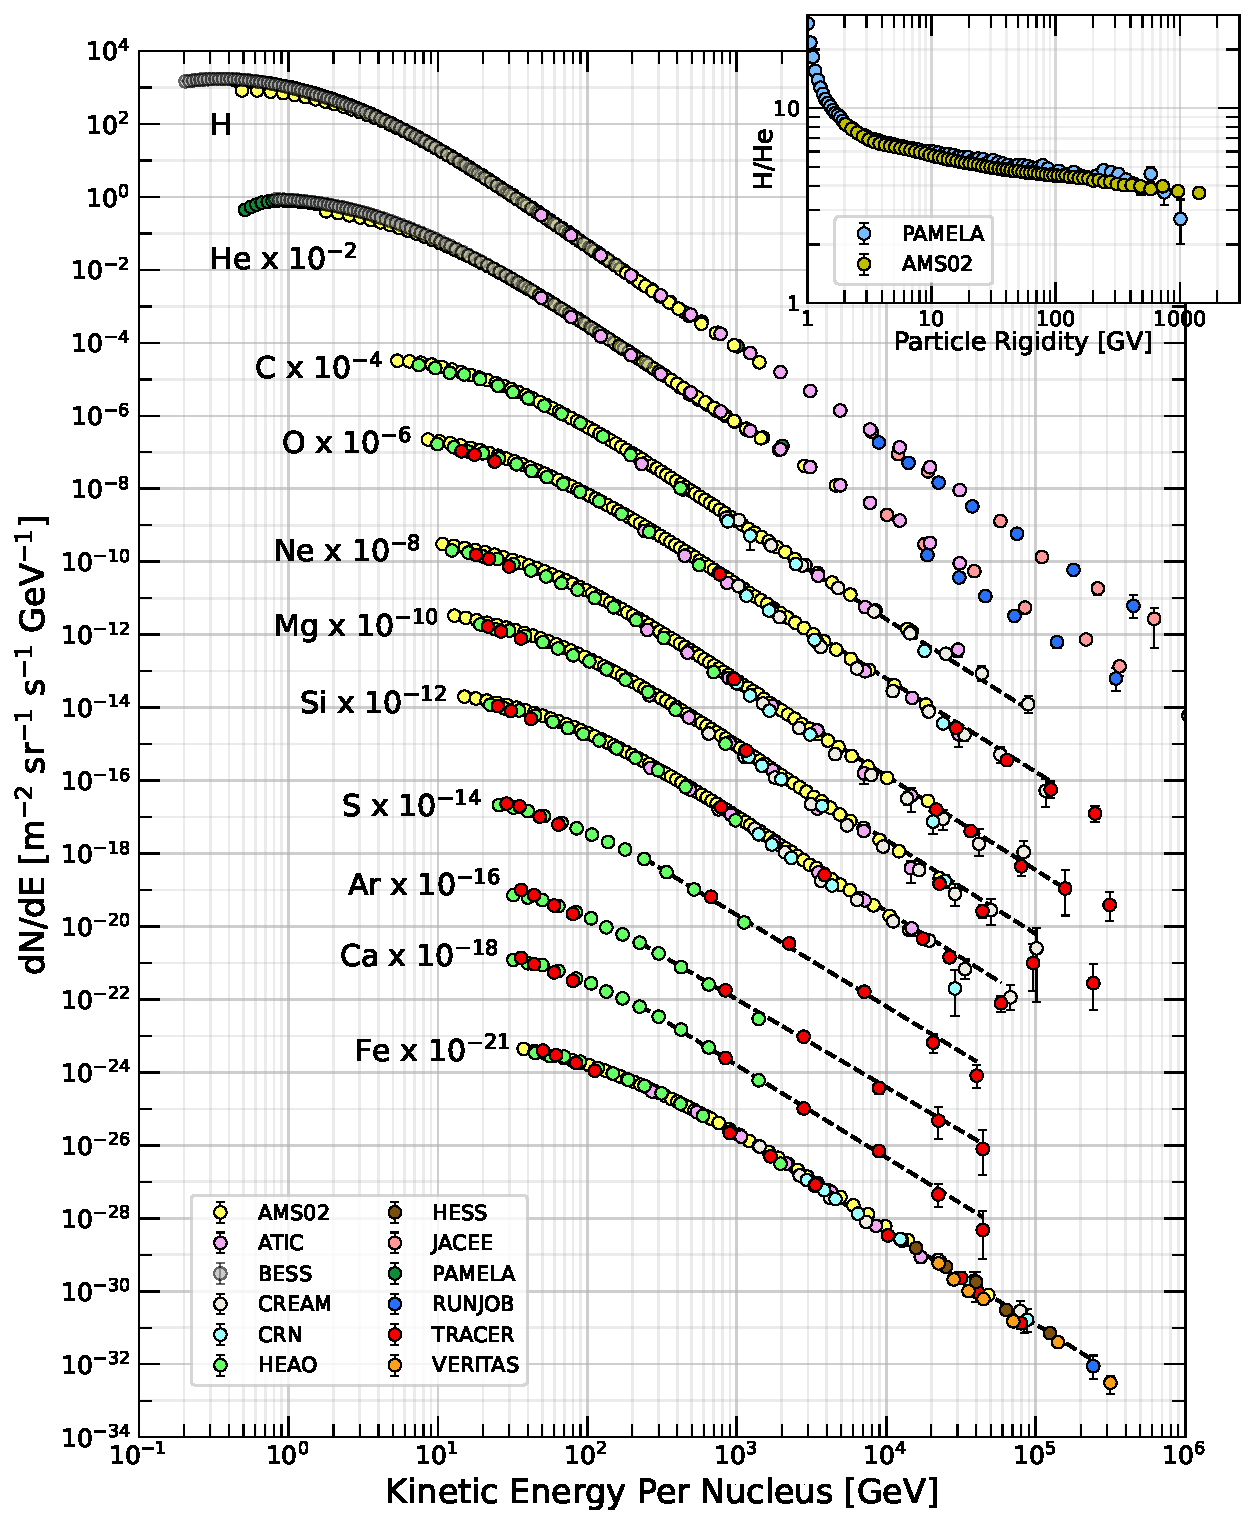
\includegraphics{figures/flux/2021_Figure_1_Inset_v1.pdf}
    \caption{Spectrum of primary cosmic rays and its components as a function of the kinetic energy. The inset shows the hydrogen to helium fraction as a function of rigidity, which is defined as the gyroradius of the ray multiplied by the magnetic field strength $R=r_L B$. Figure taken from \cite{pdg}.\label{fig:cr-primary-flux}}
\end{figure}
When a cosmic ray interacts with a nucleus, it creates a shower of hadrons that is mostly composed of Pions and Kaons that subsequently decay into muons, electrons, and neutrinos in the reaction chain
\begin{equation}
    \begin{aligned}
        \mathrm{C.R.} + N & \rightarrow X + \pi^\pm, K^\pm \\
        \pi^\pm & \rightarrow \mu^\pm + \pbar{\nu}_\mu \\
        \mu^\pm & \rightarrow e^\pm + \pbar{\nu}_e + \pbar{\nu}_\mu\;.
    \end{aligned}
\end{equation}
At energies of $\order{\SI{1}{GeV}}$, these reactions lead to a production of muon neutrinos and electron neutrinos at a ratio of $2:1$. As the energy increases, however, muons can increasingly reach the surface of the Earth and interact before they can decay, which increases the relative fraction of muon neutrinos as shown in \reffig{flux-numu-ratio}. Between GeV and TeV energies, the $\nu_\mu$ flux has a spectral index that is similar to that of the primary cosmic rays at $\gamma \approx 2.7$ as can be seen in \reffig{flux-alldir}, while the spectrum for electron neutrinos falls off more quickly at higher energies. Tau neutrinos can also be produced if a cosmic ray interaction produces charmed mesons, but such interactions are rare and the atmospheric tau neutrino flux is below 0.1\% for the energies considered in this work\cite{fedynitch2015calculation} and is therefore neglected.
\begin{figure}
\centering
\begin{subfigure}[t]{0.55\linewidth}
    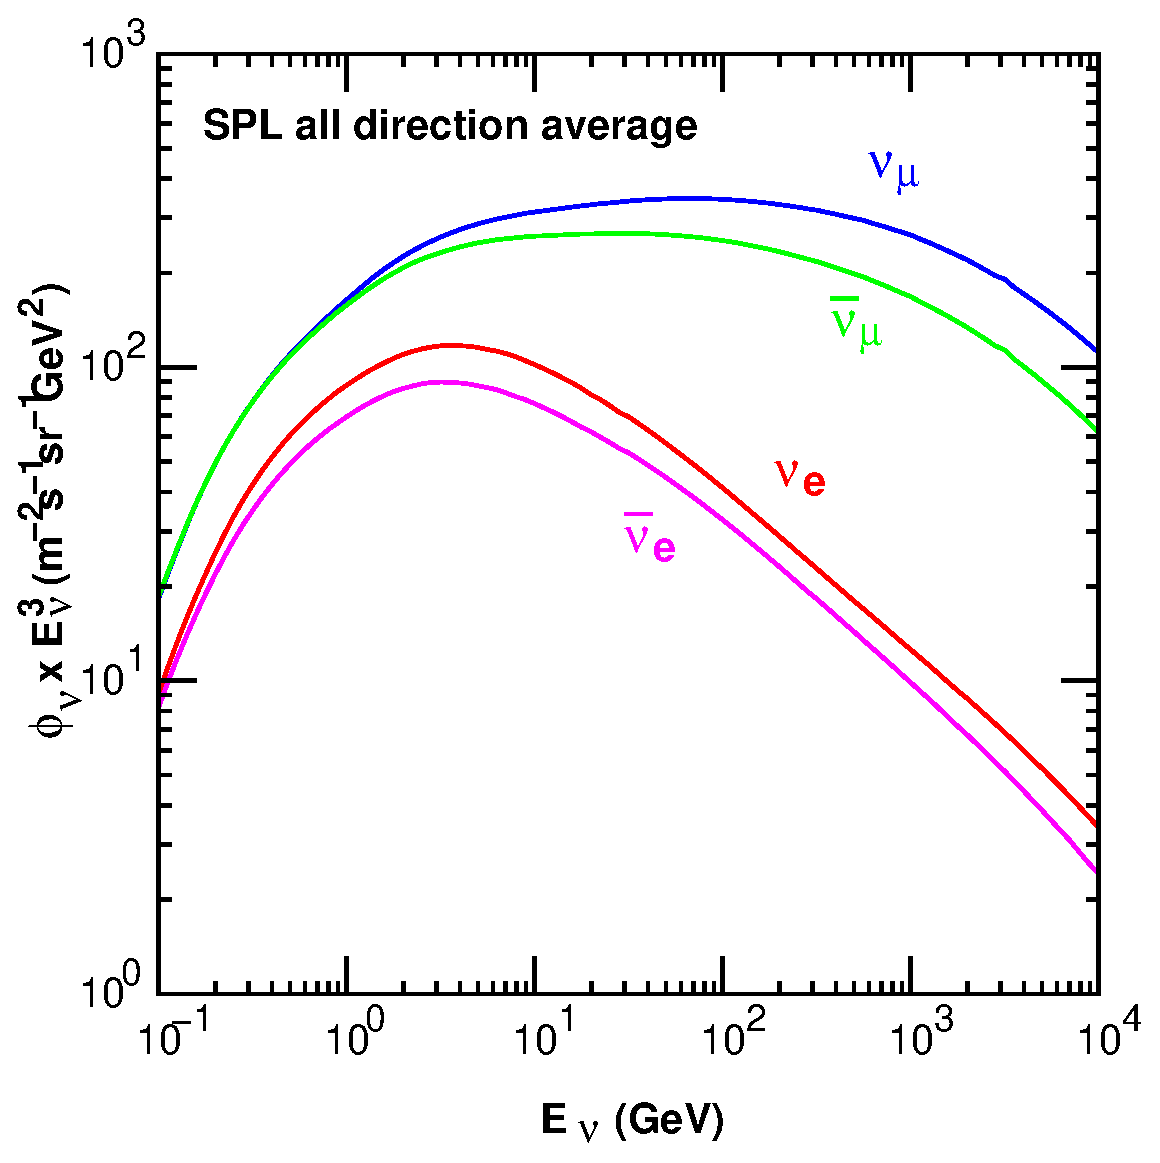
\includegraphics[height=2.2in]{figures/flux/alldir-spl.eps}
\caption{Neutrino flux averaged over all directions\label{fig:flux-alldir}}
\end{subfigure}
\hfill
\begin{subfigure}[t]{0.35\linewidth}
    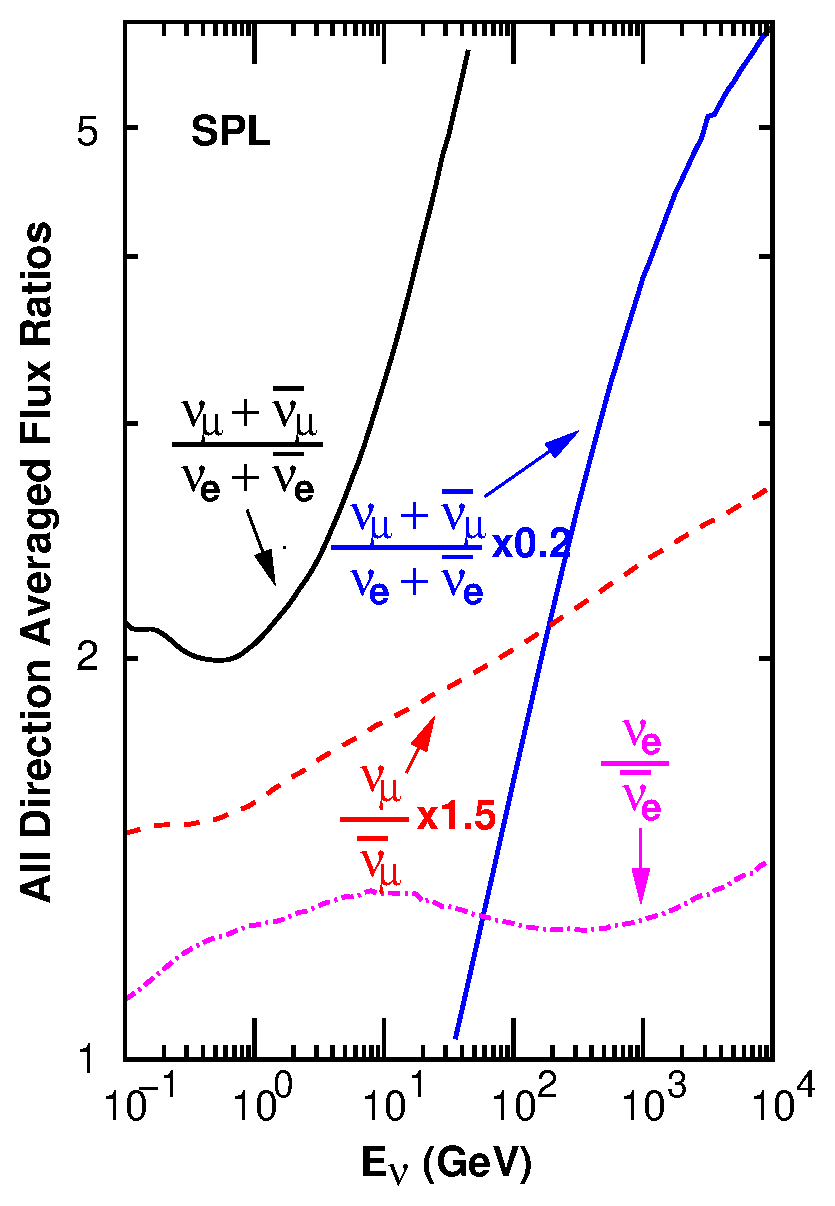
\includegraphics[height=2.2in]{figures/flux/spl-ratio-ally.eps}
\caption{Ratio of muon neutrinos to electron neutrinos\label{fig:flux-numu-ratio}}
\end{subfigure}
\caption{Neurino flux at the South Pole, averaged over all directions. Figures taken from \cite{Honda:2015fha}.}
\end{figure}

\subsubsection{Three-flavor oscillations of atmospheric neutrinos}
After neutrinos are produced in the atmosphere, they travel through the Earth before they are detected at the South Pole. Depending on the zenith angle at which a neutrino is observed, it has travelled a total distance, $L$, that depends on the radius of the Earth, $R_\oplus$, the depth of the detector, $d_\mathrm{det}$, and the production height of the neutrino, $h_\mathrm{atm}$, as illustrated in \reffig{atmo-baseline-illustration}. From the geometry, $L$ is calculated as
\begin{equation}
    L = (d - R_\oplus)\cos(\theta_z) + \sqrt{(R_\oplus + h_\mathrm{atm})^2 - (R_\oplus - d)^2\sin^2(\theta_z)}\;.\label{eq:prop-distance}
\end{equation}
\begin{figure}
    \centering
    \tikzsetnextfilename{atmo_baseline_illustration}%
\begin{tikzpicture}
    \def\Rearth{2.6}
    \def\Rcore{1.3}
    \def\Ratmo{3}
    \def\detpos{-2.2}
    \draw[name path=atmo, fill=cyan!50!white] (0,0) circle (\Ratmo);
    \shadedraw[
        outer color=brown!70!black,
        inner color=brown!40!white,
        name path=earh,
        %postaction={decorate},
        %decoration={raise=2pt, text along path, text={Earth}, text align=center}
    ] (0,0) circle (\Rearth);
    \shade[outer color=brown!70!black,inner color=brown!40!white, name path=earh] (0,0) circle (\Rcore);
    \node [draw, thick, shape=rectangle, minimum width=0.3cm, minimum height=0.4cm, anchor=center, fill=gray] (detector) at (0, \detpos) {};
    \path [name path=nupath] (detector) +(55:6) -- +(235:1);
    \draw [name intersections={of=nupath and atmo, by={a,b}}, -stealth, very thick] (a) -- node[above, sloped] {$L$} (b);
    \draw [name intersections={of=nupath and atmo, by={a,b}}, thick] (detector.center) --  node [sloped, above, pos=0.6] {$R_\oplus - d_\mathrm{det}$} (0,0) -- node [sloped, above] {$R_\oplus + h_\mathrm{atm}$} (a);
    \draw (detector) +(90:0.4) arc (90:235:0.4) node[midway, anchor=east] {$\theta_z$};
    \draw [stealth-stealth] (0,0) -- node [above] {$R_\oplus$} (150:\Rearth);
    \draw [stealth-stealth] (150:\Rearth) -- node [draw,above=0.2cm, fill=white] {$h_\mathrm{atm}$} (150:\Ratmo);
    \draw (detector.center) -- (detector -| 0.5,0);
    \draw (0, -\Rearth) -- (0.5, -\Rearth);
    \draw [stealth-stealth] (0.5, -\Rearth) -- node[draw, fill=white, right=.1cm] {$d_\mathrm{det}$} (detector -| 0.5,0);
    \node [anchor=north] at (0,\Rearth) {\footnotesize mantle};
    \node [anchor=north] at (0,\Rcore) {\footnotesize core};
\end{tikzpicture}

    \caption{Illustration of the geometry of atmospheric oscillation measurements. The detector is shown as the gray box near the bottom and $\theta_z$ indicates the observed zenith angle of a neutrino.\label{fig:atmo-baseline-illustration}}
\end{figure}
If the height of the atmosphere and detector depth is neglected, \refeq{prop-distance} reduces to
\begin{equation}
    L =
    \begin{cases}
        0 & \theta_z \leq \frac{\pi}{2} \\
        2 R_\oplus \cos \theta_z & \theta_z > \frac{\pi}{2}
    \end{cases}\;.
\end{equation}
From the perspective of the IceCube detector, an \emph{up-going event} is one where the zenith angle is $\theta_z > \ang{90}$, that is, $\cos(\theta_z) < 0$. On the other hand, a \emph{down-going} event is one where $\cos(\theta_z) > 0$. In such cases, the neutrino travels only through the atmosphere and the overburden of the detector and therefore matter effects are negligible.  The Earth is modeled as a set of concentric shells with different matter densities. The most prominent feature in the density profile is the core region at a depth of close to half an Earth radius, where the density sharply increases from \SI{5}{\gram\per\centi\meter\cubed} to \SI{>10}{\gram\per\centi\meter\cubed}\cite{PREM}. Neutrinos for which $\cos(\theta_z) \lesssim 0.8$ travel partially through the core and generally experience greatly enhanced matter effects. Given the baseline of $\order{R_\oplus\sim\SI{e4}{km}}$ and the core energy range of the atmospheric neutrino spectrum between GeV and TeV scales, the mass splitting between mass eigenstates whose oscillation could be observed $\SI{e-4}{eV^2} < \Delta m^2 < \SI{e-1}{eV^2}$.

Since the primary constituent of the atmospheric neutrino flux are muon (anti-)neutrinos, the most important oscillation channel to be observed is the muon neutrino survival probability.\todo{more detail on phenomenology of atmospheric oscillations}

\subsection{Accelerator neutrinos}
The $\nu_\mu \rightarrow \nu_\mu$ oscillation channel probed by atmospheric neutrino oscillations is also accessible via long-baseline accelerator neutrino experiments. These experiments use neutrinos that are produced when protons are shot at a stationary target by a particle accelerator. The interactions of the protons with the target produce a hadronic shower consisting mostly of pions that are then focused into a tube where they are allowed to decay into neutrinos and charged leptons. This process is very similar to the production of neutrinos in the atmosphere and leads to a beam that is composed of mostly muon neutrinos and some electron neutrinos. The beam is targeted at a detector that is typically located several hundreds of kilometers away from the neutrino production site. An example for such an experimental setup is the MINOS experiment\cite{MICHAEL2008190}. \reffig{numi-beam} shows the setup of the Neutrino Main Injector (NuMI) that produces neutrinos for MINOS at a peak energy of \SI{3}{GeV}. The neutrino flux is measured at a near and a far detector at baselines of \SI{1}{km} and \SI{735}{km}, respectively, that are both identically constructed magnetized steel-scintillator tracking calorimeters. The atmospheric mass splitting and mixing angle can be estimated by comparing the neutrino flux at the near and far detectors, such that most of the inherent systematic uncertainties of the measurement cancel out. Other experiments with a similar setup are T2K\cite{T2K:2011qtm} and NO$\nu$A\cite{Patterson:2012zs}.
\begin{figure*}
    \centering
    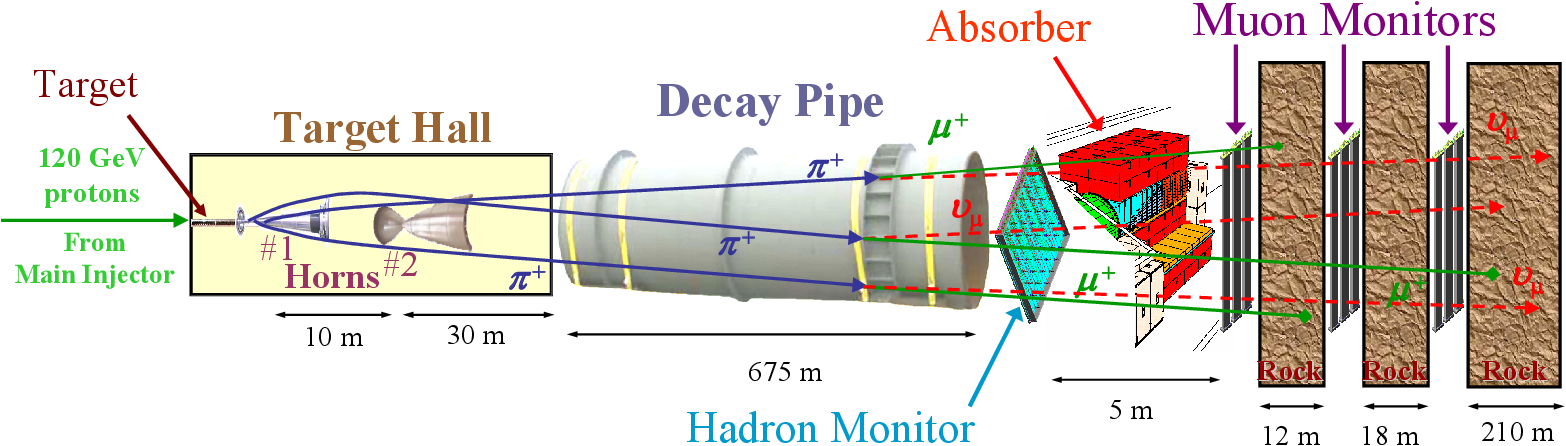
\includegraphics{figures/theory/numi_beam.png}
    \caption{Neutrino Main Injector (NuMI) facility producing neutrinos for the MINOS experiment. Figure taken from\cite{osti_879065}.\label{fig:numi-beam}}
\end{figure*}

\section{Anomalies in neutrino oscillation measurements}
While the three-flavor oscillation picture explains most of the experimental data from reactor, accelerator, atmospheric and solar neutrino experiments fairly well, there are some notable exceptions of anomalous experimental observations. These anomalies are
\begin{itemize}
    \item Reactor Antineutrino Anomaly: A deficit of $\bar{\nu}_e$ in the neutrino flux of nuclear reactors with respect to the theoretical flux expectation at baselines between $L\sim\SI{10}{m}$ and $L\sim\SI{100}{m}$.
    \item Gallium anomaly: A deficit of $\nu_e$ in the flux of a radioactive $^{51}\mathrm{Cr}$ source. The detector is in direct contact with the source and is of $\order{\SI{1}{m}}$ in size in each dimension.
    \item LSND anomaly: An excess of $\bar{\nu}_e$ in the neutrino flux of a proton-on-target (accelerator) source at $L\sim\SI{30}{m}$ and $E\sim\SI{30}{MeV}$.
    \item MiniBooNE anomaly: Excess of electron-like events in the the flux of neutrinos generated by an accelerator source at $L\sim\SI{500}{m}$ and $E\sim\SI{500}{MeV}$.
\end{itemize}
This section summarizes each of these measurements and describes how they could be resolved by the introduction of sterile neutrino states.

\subsection{Reactor neutrino anomaly}
The Reactor Antineutrino Anomaly (RAA) was first described in 2011\sidecite{Mention:2011rk} after new corrections were introduced into the theoretical calculations to the predicted neutrino flux from commercial nuclear reactors. The corrections adjusted the predicted flux upwards, leaving a deficit of $\sim 6\%$ in the measured flux with respect to the new prediction. It is suggested in \cite{Mention:2011rk} that this deficit could be explained by the introduction of an additional mass eigenstate with a mass splitting, $\Delta m^2_{41}$, and mixing angle, $\theta_{14}$. The electron neutrino survival probability can be approximated for distances of $L\lesssim \SI{1}{km}$ as
\begin{equation}
    P_{ee} = 1 - \cos^4 (\theta_{14}) \sin^2 (2\theta_{13}) \sin^2 \left(\frac{\Delta m^2_{31} L}{4E} \right) - \sin^2 (2\theta_{14}) \sin^2 \left(\frac{\Delta m^2_{14} L}{4E} \right)\;.\label{eq:approx-Pee}
\end{equation}
The magnitude of the additional mass splitting and mixing angle proposed in \cite{Mention:2011rk} is $\abs{\Delta m^2_{41}} \gg \SI{1}{eV^2}$ and $\sin^2(2\theta_\mathrm{new})=0.12$, respectively. The oscillations due to this mass eigenstate would be too fast to be resolvable and would only lead to an average deficit that is shown as the blue line in \reffig{raa}. The red line shows the flux expectation in the presence of only three active flavors.
\begin{figure}
    \centering
    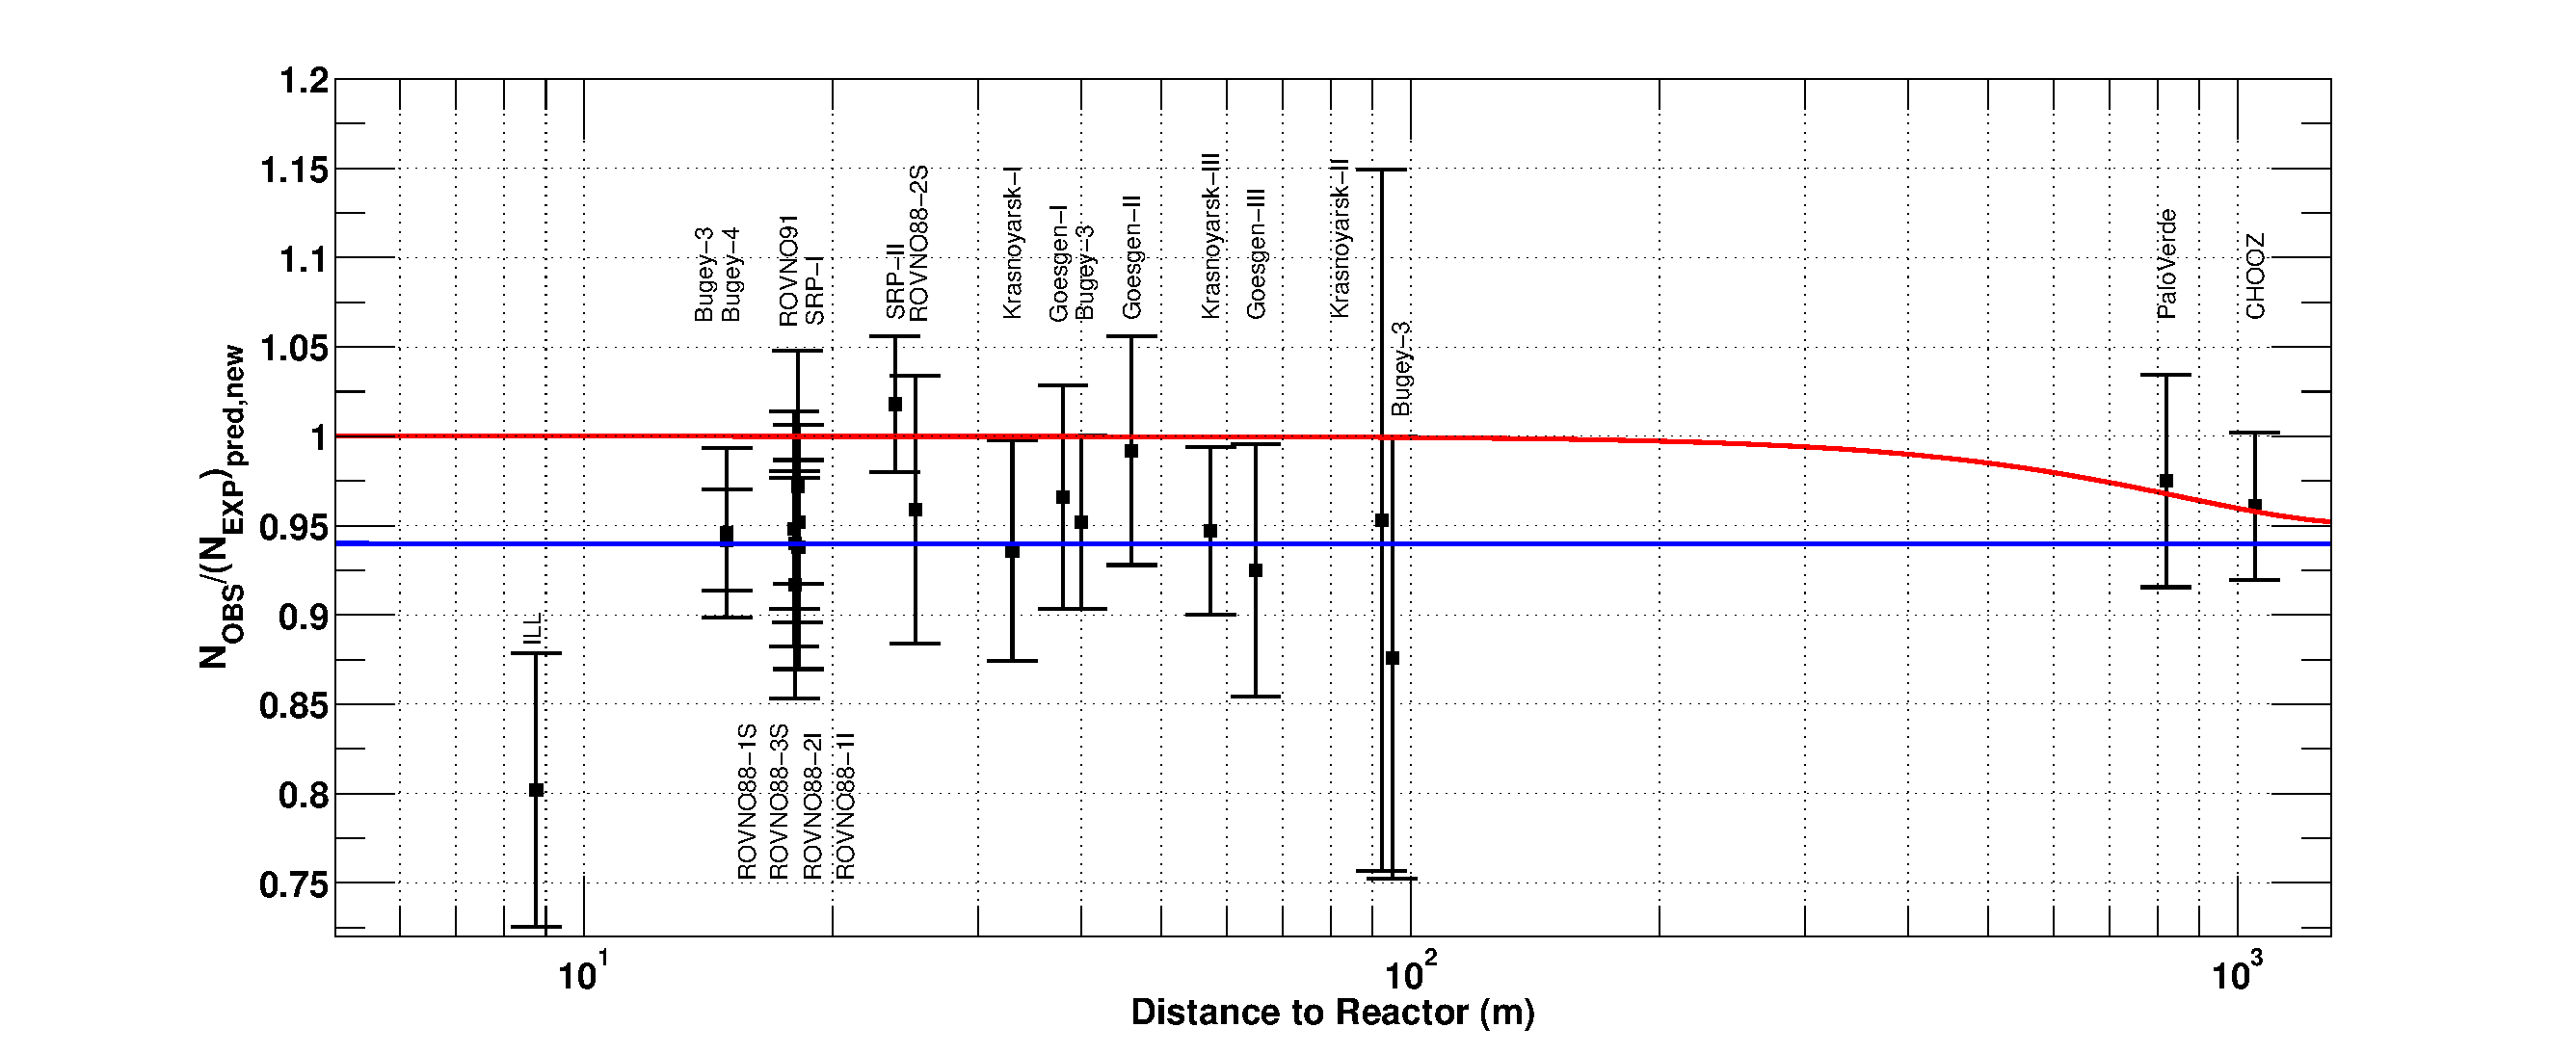
\includegraphics{figures/theory/raa.pdf}
    \caption{Deficit in $\bar{\nu}_e$ flux from commercial nuclear reactors referred to as Reactor Antineutrino Anomaly. Figure taken from \cite{Mention:2011rk}.\label{fig:raa}}
\end{figure}
\begin{marginfigure}
    \centering
    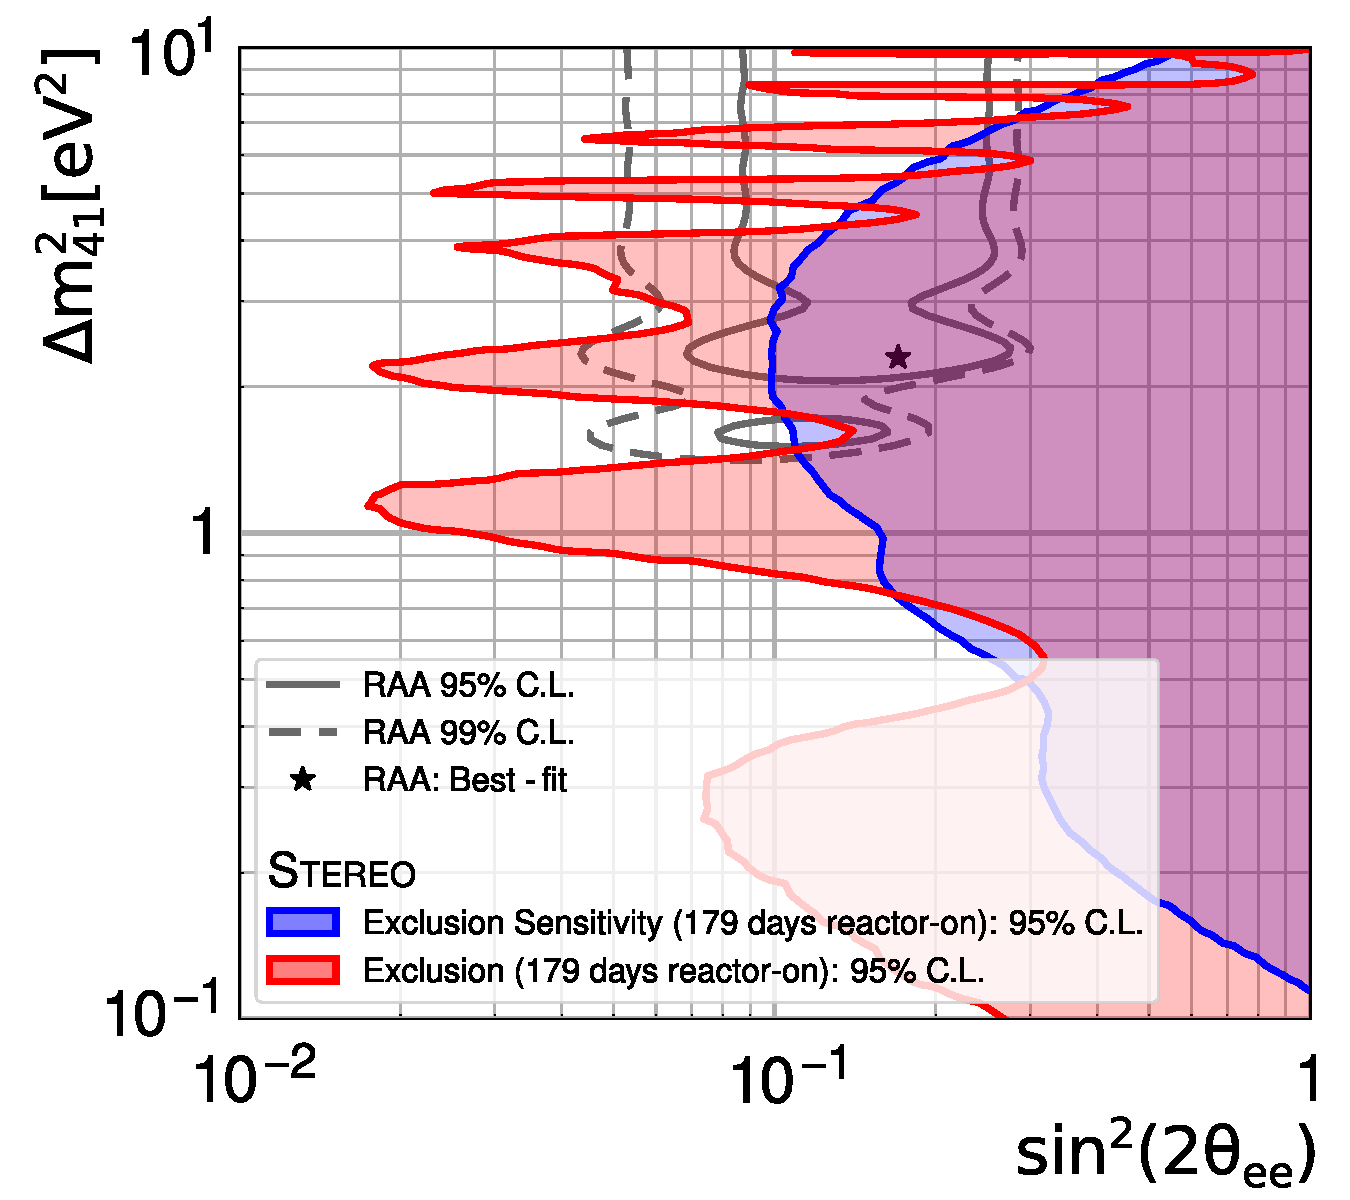
\includegraphics{figures/theory/ST_osc.pdf}
    \caption{Exclusion contours for the sterile mass splitting and mixing angle from the \textsc{STEREO} experiment. The effective mixing angle $\theta_{ee}$ is equivalent to $\theta_{13}$ in \refeq{approx-Pee}. Red shaded areas are excluded by the measurement at 95\% C.L., blue shaded areas are the estimated 95\% sensitivity. Gray solid lines show the preferred values of the RAA. Figure taken from \cite{Licciardi:2021hyi}.\label{fig:sterile-exclusions-stereo}}
\end{marginfigure}
Whether or not the RAA truly is an anomaly depends on whether or not one trusts the theoretical flux predictions. The involved calculations require complex nuclear corrections that are not perfectly understood. The RAA is in fact not the only anomaly in the reactor antineutrino flux. The second anomaly, an excess of $\bar{\nu}_e$ at $\sim \SI{5}{MeV}$, is thought to originate from poorly understood nuclear physics\cite{HUBER2016268}. For this reason, the RAA was put under scrutiny by follow-up experiments that only measure flux differences between different baselines to cancel uncertainties in the absolute flux. Three such experiments are STEREO, PROSPECT, and DANSS. The detectors of STEREO and PROSPECT are segmented between baselines of respectively \SIrange{9.4}{11.2}{m} and \SIrange{6.7}{9.3}{m}, while the DANSS detector is positioned on a movable platform that allows for measurements to be taken at baselines of \SIlist{10.9;11.9;12.9}{m}\sidecite{Licciardi:2021hyi}. The results of the measurements of these three experiments show no sign of baseline-dependent flux variations and thereby exclude the oscillation amplitude preferred by the RAA at mass splitting values between \SI{0.1}{eV^2} and \SI{10}{eV^2}. The contours for \textsc{STEREO} are shown in \reffig{sterile-exclusions-stereo}, those for \textsc{DANSS} and \textsc{PROSPECT} look very similar and can be found in \cite{Licciardi:2021hyi}. However, these measurements still allow oscillations due to a mass eigenstate with $\Delta m^2_{41}> \SI{10}{eV^2}$ that cannot be resolved by their detector segmentation. More recent reevaluations of the reactor flux model in light of new data from the research reactor in National Research Centre Kurchatov Institute (KI) have increased the predicted flux again and thereby resolved the anomaly almost entirely\sidecite{Giunti_2022}.

\subsection{Gallium anomaly}
\begin{marginfigure}
    \centering
    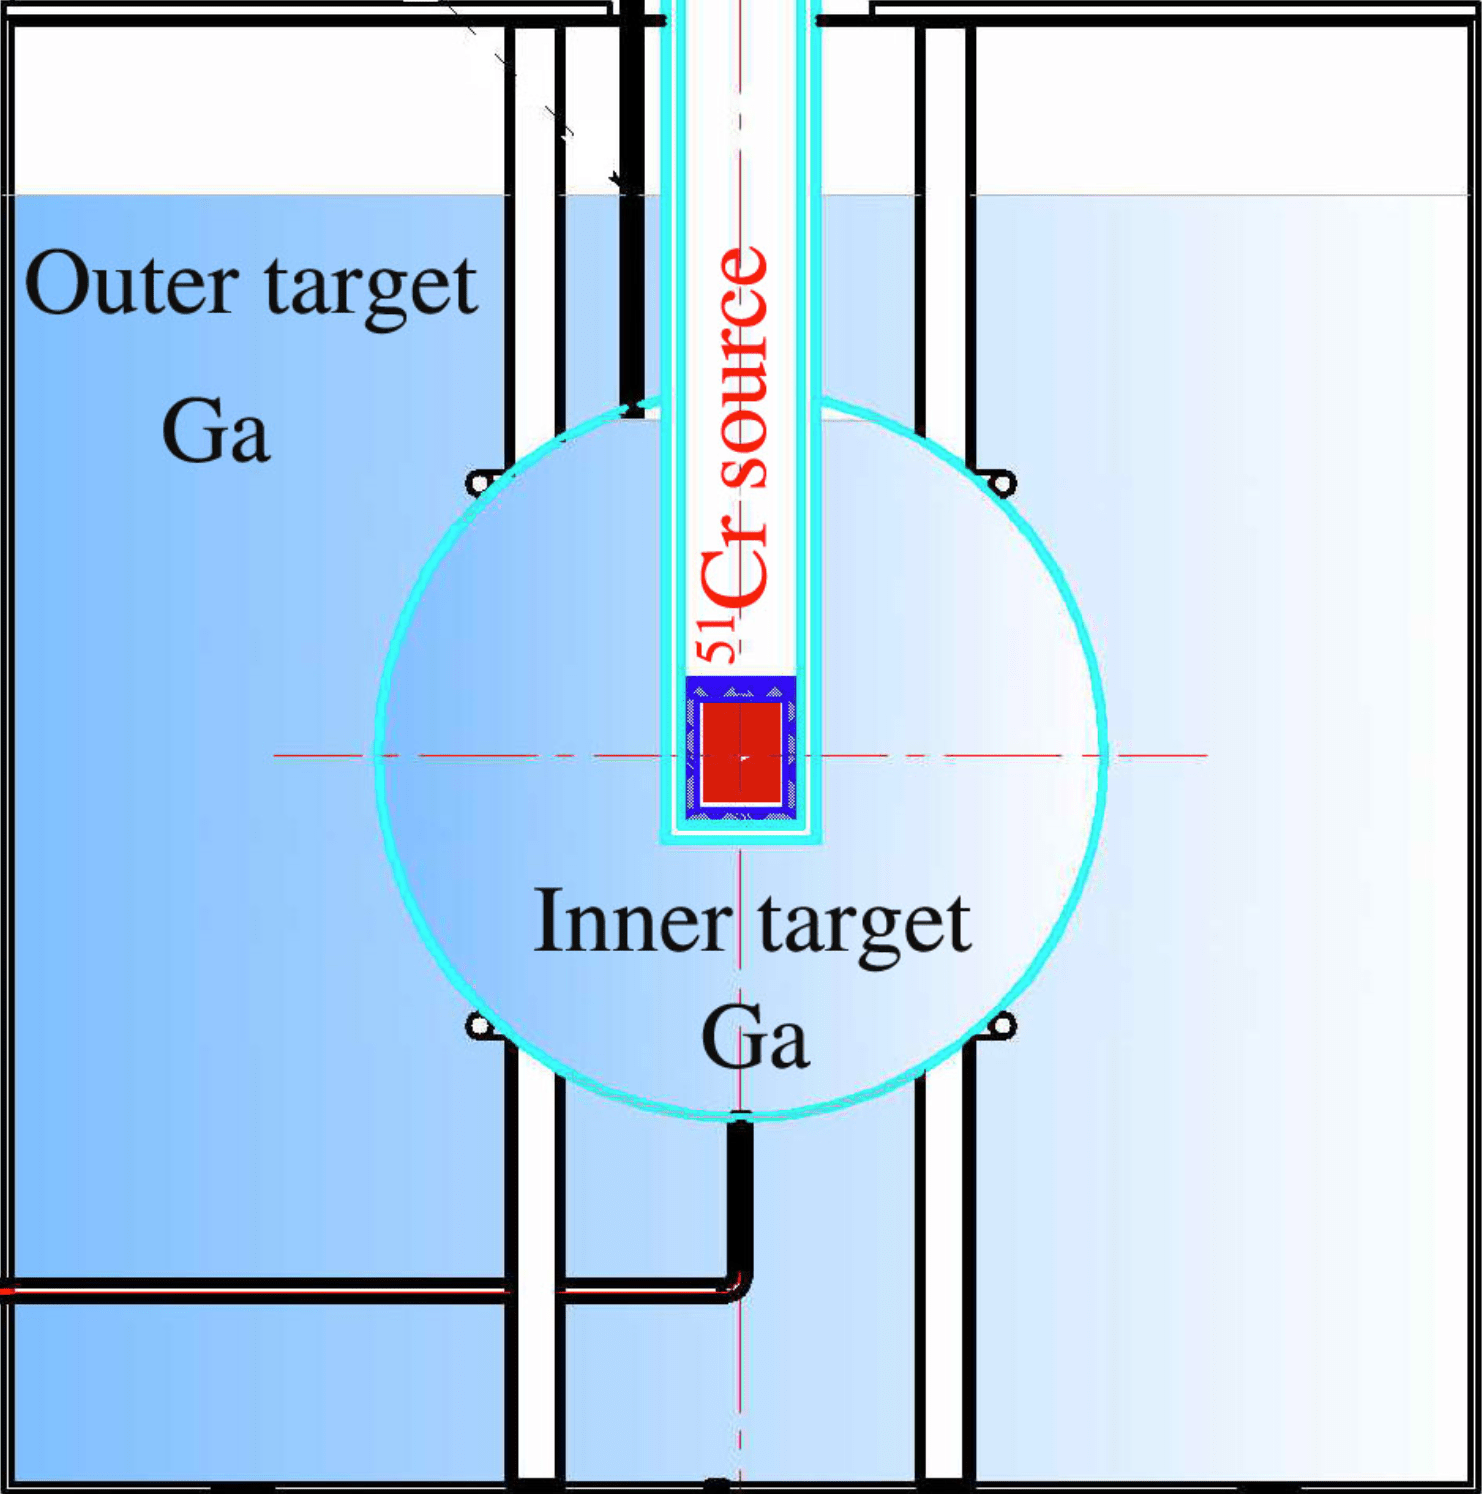
\includegraphics{figures/theory/BESTscheme_cropped_small.png}
    \caption{Experimental setup of the BEST experiment. The diameters of the inner and outer volumes are \SI{133.5}{cm} and \SI{218}{cm}, respectively. Figure taken from \cite{Barinov_2022}.\label{fig:best-experiment}}
\end{marginfigure}
The Gallium anomaly is a relatively large ($\sim20\%$) deficit of electron-neutrinos observed in measurements of the flux from a $^{51}\mathrm{Cr}$ source at very short distances that was first observed in the GALLEX experiment\cite{gallex:1998} and that has been more recently confirmed by the SAGE and BEST experiments\cite{Barinov_2022,Abdurashitov_2006}.The BEST experiment consists of an inner and outer detector volume surrounding the radioactive source as shown in the diagram in \reffig{best-experiment}, such that the flux can be compared at two different baselines. The measured ratios in the outer and inner volumes are, respectively, $R_\mathrm{out} = \num{0.77+-0.05}$ and $R_\mathrm{in} = \num{0.79+-0.05}$. These results do not demonstrate any baseline-dependent effects, but they are consistent with the overall deficit observed by SAGE and GALLEX. The weighted average ratio between the expected and predicted flux of all three experiments is $R=\num{0.8+-0.05}$, which brings the significance of the Gallium anomaly to $4\sigma$. In order to explain this ratio with a two-flavor $\nu_e \rightarrow \nu_s$ oscillation model, the mass splitting would have to be $\Delta m^2 > \SI{1}{eV^2}$ such that the oscillations would average out between the inner and outer volumes of the BEST experiment, and the mixing angle would have to be rather large at $\sin^2(2\theta)\approx 0.4$. This large amount of mixing puts the Gallium anomaly in tension with the reactor anomaly, in particular in light of the more recent flux calculations. The $2\sigma$ contours for the effective mixing parameters of both anomalies are shown in \reffig{best-contours}. The reactor anomaly results are shown for different flux models described in \cite{Giunti_2022}. Notably, the contour using the the KI and EF flux models are not closed and are therefore compatible with the null hypothesis of no sterile mixing. The gallium anomaly is shown for different cross-section models. The contours are all closed, suggesting that uncertainties in the cross-section calculation cannot resolve the gallium anomaly.
\begin{figure}
    \centering
    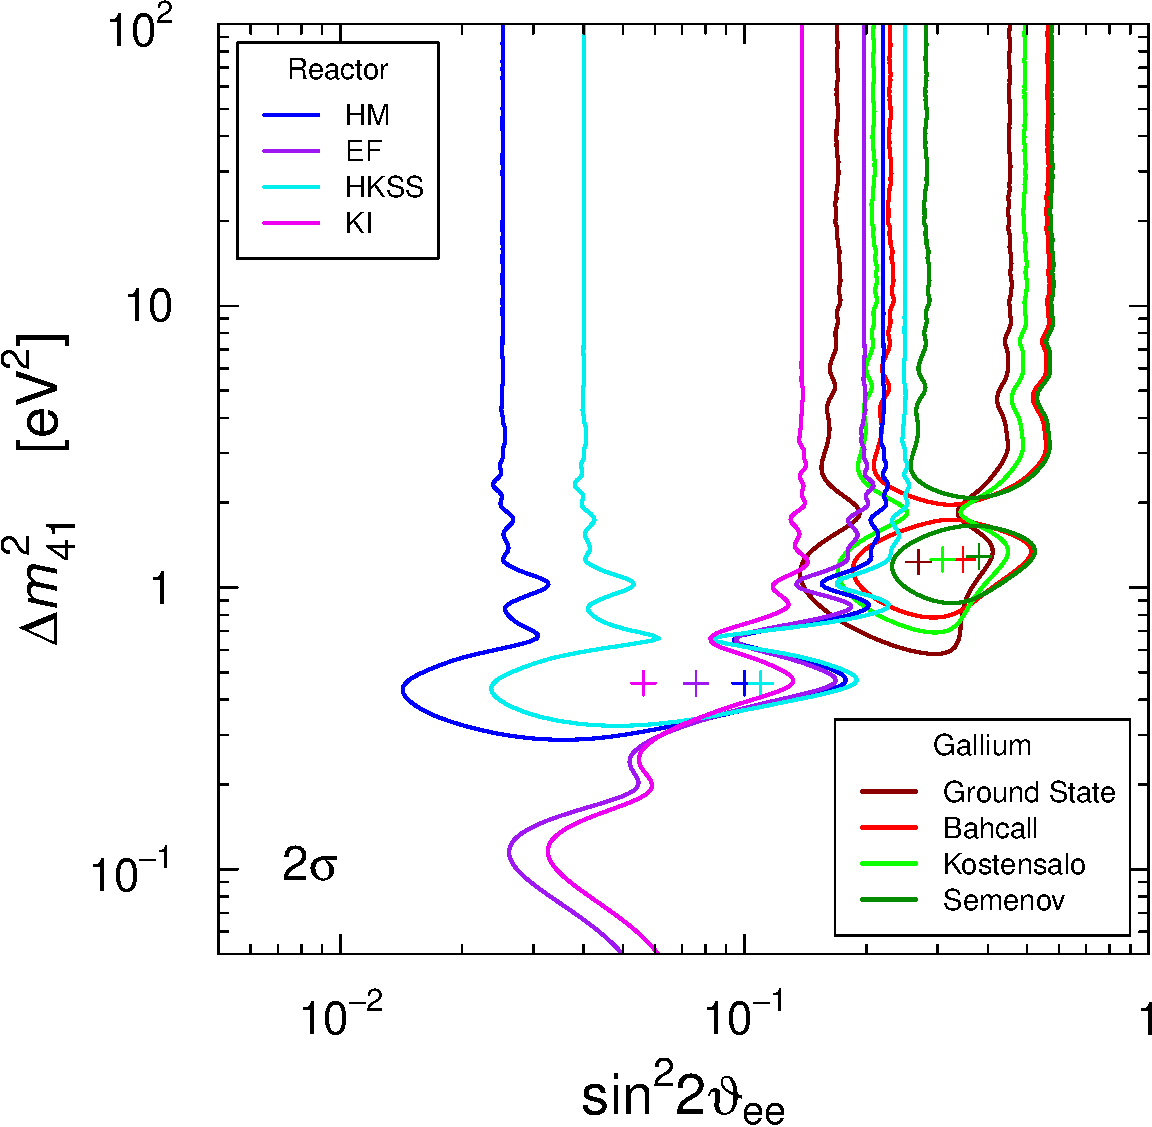
\includegraphics[width=0.7\linewidth]{figures/theory/see-gal-rat-2s.pdf}
    \caption{Contours delimiting the $2\sigma$ allowed regions of the Gallium anomaly and the reactor anomaly in mass splitting and the effective mixing angle $\sin^2(2\theta_{ee}) = 4 (1-|U_{e4}|^2)|U_{e4}|^2$. The reactor contours are shown for different flux predictions and the Gallium anomaly contours are shown under different neutrino cross-section models. Figure taken from \cite{Giunti_2022}.\label{fig:best-contours}}
\end{figure}

\subsection{LSND and MiniBooNE Anomalies}
\begin{marginfigure}
    \centering
    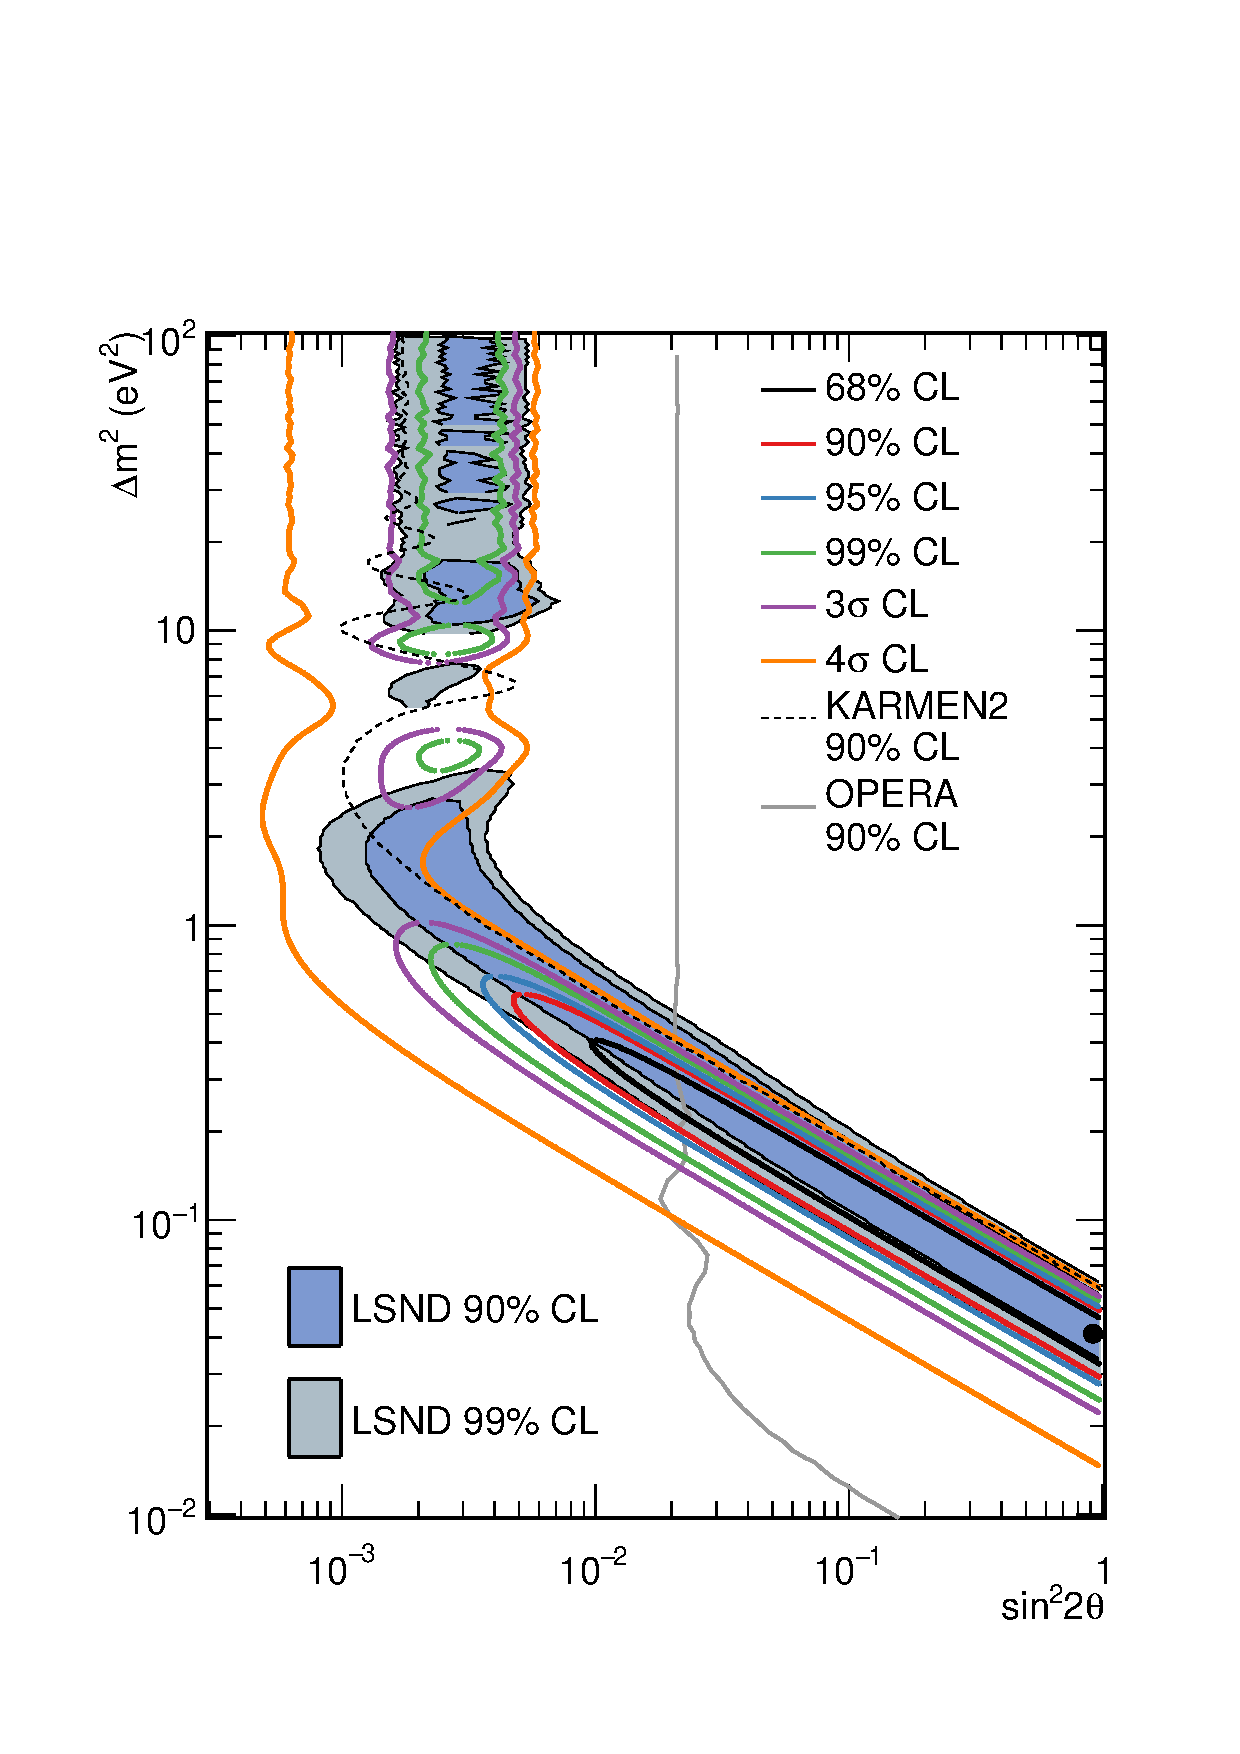
\includegraphics{figures/theory/miniboone_fake_apr18_contNunubar_with_karmen_opera.pdf}
    \caption{MiniBooNE allowed regions for a combined neutrino and antineutrino dataset within a two-neutrino oscillation model.  The shaded areas show the 90\% and 99\% C.L. LSND $\bar{\nu}_{\mu}\rightarrow\bar{\nu}_e$ allowed regions. Figure taken from \cite{MiniBooNE:2018esg}.\label{fig:miniboone-lsnd-regions}}
\end{marginfigure}
Both the LSND and MiniBooNE anomalies are unexplained excesses in the $\bar{\nu}_e$ flux of accelerator-generated neutrinos. The LSND measurement found a $3.8\sigma$ excess at a baseline of  $L\sim\SI{30}{m}$ and neutrino energy $E\sim\SI{30}{MeV}$\cite{LSND:2001aii}. The MiniBooNE experiment was set up specifically to probe the parameter space of the LSND result at a very different baseline and energy, where the systematic uncertainties would be different. It found a $4.5\sigma$ excess at \cite{MiniBooNE:2018esg} at a baseline of $L\sim\SI{500}{m}$ and neutrino energy of $E\sim\SI{500}{MeV}$. The preferred regions for the mass splitting and mixing angle of both experiments are largely compatible as shown in \reffig{miniboone-lsnd-regions}. However, the two-flavor oscillation hypothesis does not seem to fit the energy distribution of the observed excess in the lowest energy bins very well, as can be seen in the histogram in \reffig{miniboone-excess-hist}. The mismatch suggests that the simple 3+1 model may not be enough to resolve the anomaly and that more complicated models such as sterile neutrinos with decay\cite{Fischer_2020} or additional ``dark sector`` interactions\cite{PhysRevLett.121.241801} might be necessary.
\begin{figure}
    \centering
    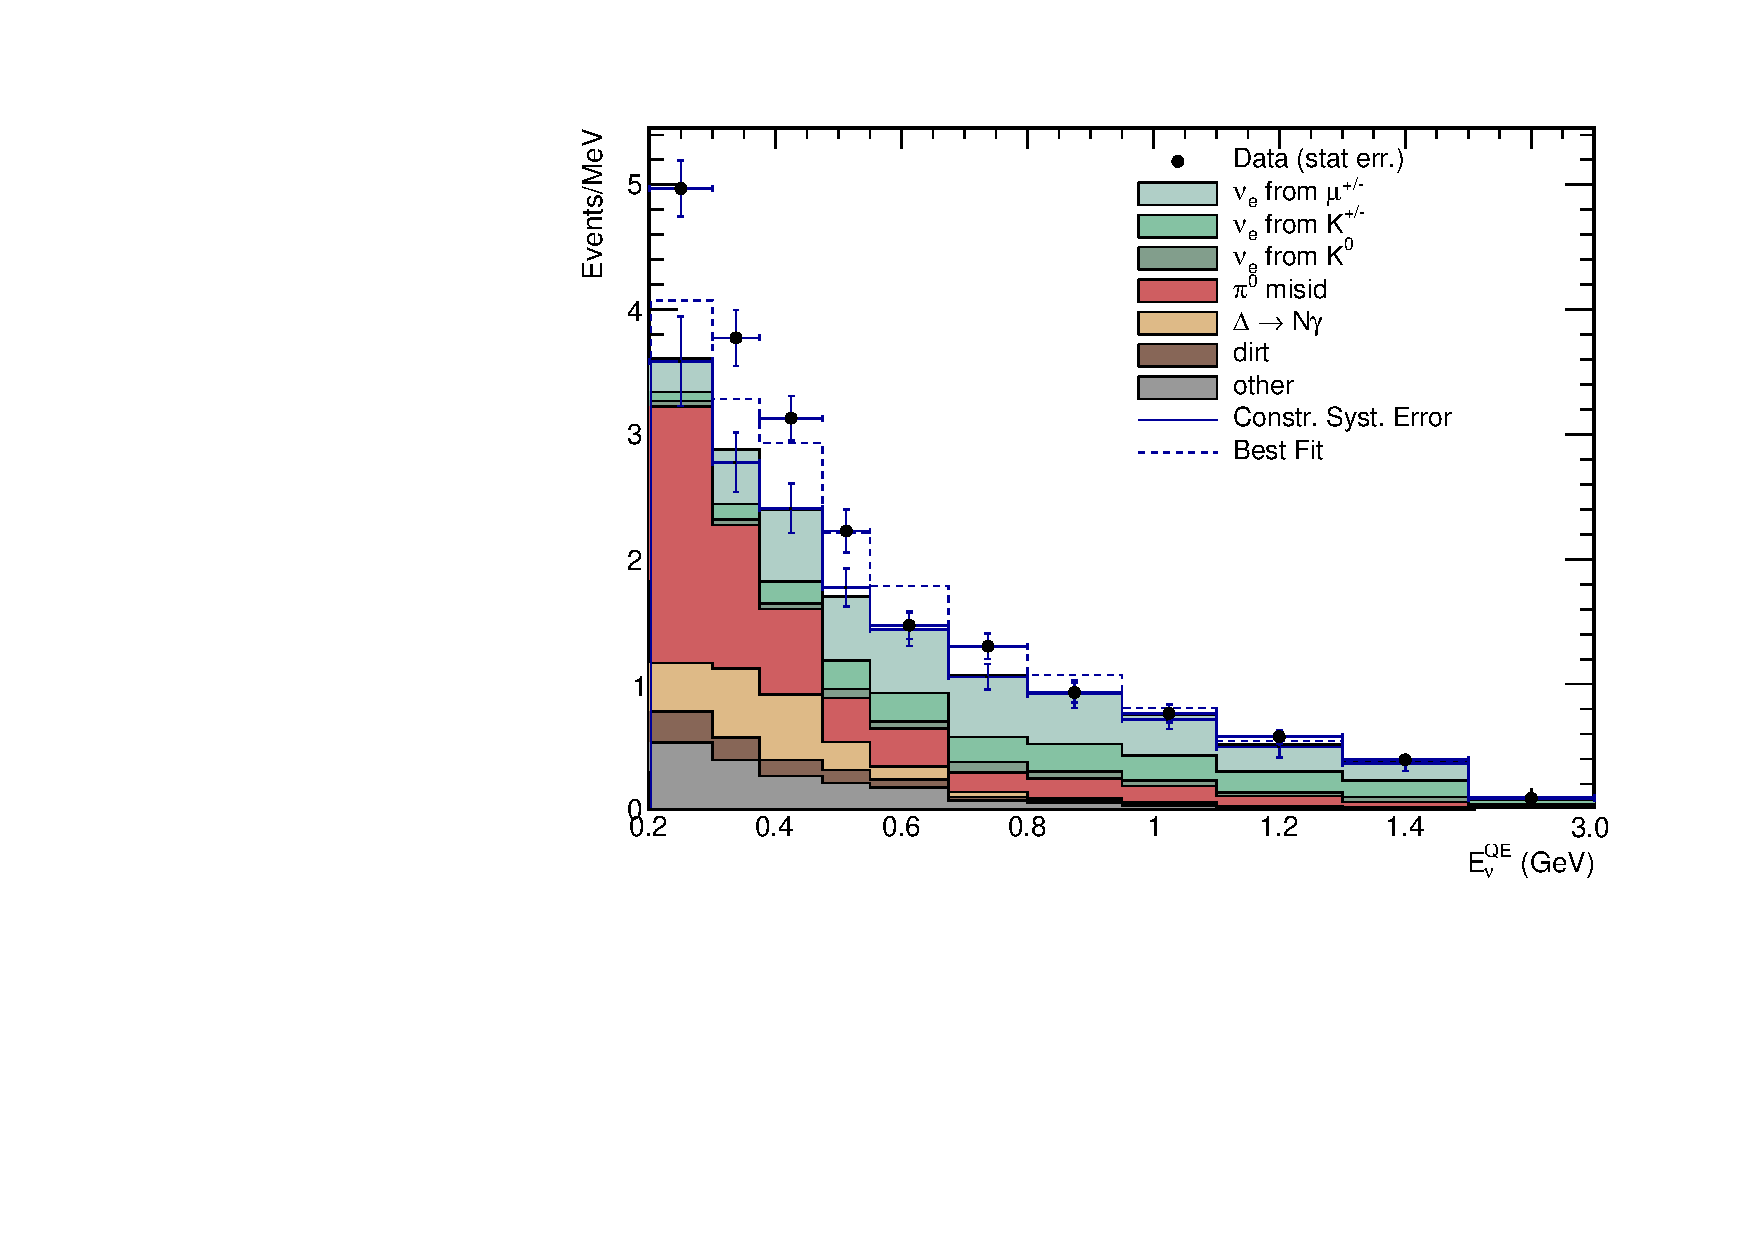
\includegraphics[width=0.8\linewidth]{figures/theory/histNu_stacked_wbf.pdf}
    \caption{MiniBooNE neutrino mode $E^{QE}_\nu$ for $\nu_e$ CCQE data (points with error bars) and background (histograms). The dashed line shows the best fit of a two-flavor oscillation hypothesis. Figure taken from\cite{MiniBooNE:2018esg}.\label{fig:miniboone-excess-hist}}
\end{figure}
The MiniBooNE excess has been measured on top of a large background dominated by photon-producing neutrino-nucleus interactions that are subject to substantial theoretical uncertainties. A more recent re-analysis of the MiniBooNE data found that a more conservative treatment of all these uncertainties reduces the magnitude of the observed excess somewhat, but leaves the significance of the sterile oscillation hypothesis still at $3.6\sigma$\cite{Giunti:2019sag}. A followup experiment, MicroBooNE\cite{MicroBooNE:2016pwy}, uses a Liquid Argon Time Projection Chamber (LiArTPC) to detect neutrino interactions. In contrast to MiniBooNE, MicroBooNE can separate interactions with electrons in the final state (that is, charged-current quasi-elastic interactions of $\nu_e$) from neutral-current interactions that produce a single photon. While recent results from MicroBooNE could exclude some of the suspected photon producing states as the culprit of the anomalous excess\cite{MicroBooNE:2021zai}, they were also not able to confirm the anomaly in the electron neutrino channel\cite{MicroBooNE:2022wdf}.

\subsection{Global picture of oscillation anomalies}
\label{sec:global-anomalies}
While some of the observed anomalies, in particular the LSND and Gallium anomalies, could be confirmed to a high significance by later experiments, it is challenging to reconcile them all in a cohesive global neutrino oscillation model. The simplest model that can be invoked in order to explain the anomalous appearances and disappearances of electron neutrinos is the addition of a fourth neutrinos mass eigenstate, $\nu_4$, and an unobservable sterile flavor eigenstate, $\nu_s$, and to allow the active neutrino flavors to oscillate into and out of the sterile state. Theoretically, such an addition is possible by adding a Majorana mass term as described in \refsec{neutrino-masses}. The flavor and mass eigenstate would then mix via an extended "3+1" mixing matrix
\begin{equation}
    \begin{pmatrix}
        \nu_e \\ \nu_\mu \\ \nu_\tau \\ \nu_s
    \end{pmatrix}
    =
    \begin{pmatrix}
    U_{e1}    & U_{e2}    & U_{e3}   &U_{e4}    \\
    U_{\mu1}  & U_{\mu2}  & U_{\mu3} &U_{\mu4}  \\
    U_{\tau1} & U_{\tau2} & U_{\tau3}&U_{\tau4} \\
    U_{s1} & U_{s2} & U_{s3}&U_{s4} \\
    \end{pmatrix}
    \begin{pmatrix}
        \nu_1 \\ \nu_2 \\ \nu_3 \\ \nu_4
    \end{pmatrix}
\end{equation}
and the fourth mass eigenstate would be much heavier than the first three states with a mass splitting of $\Delta m^2_{41} \gg \Delta m^2_{31}$. Because the oscillations due to this additional mass eigenstate would be much faster than those of the active flavors, the transition probability between flavors $\alpha$ and $\beta$ can be described in the two-flavor approximation
\begin{equation}
    P_{\alpha\beta}\simeq \delta_{\alpha\beta} - 4\abs{U_{\alpha\beta}}^2(\delta_{\alpha\beta}-\abs{U_{\alpha\beta}}^2)\sin^2\left(\frac{\Delta m^2_{41}L}{4E}\right)\;.
\end{equation}
It is convenient to define effective mixing angles for each oscillation channel that is probed by different experiments as listed in \reftab{effective-mixing-definitions}. Since there are three measurable mixing angles that depend on only two matrix elements, the model can be over-constrained by measurements of $\theta_{\mu 3}$, $\theta_{ee}$ and $\theta_{\mu\mu}$.
\begin{table}
    \caption{Definitions of effective mixing angles in the "3+1" oscillation model for oscillation channels relevant to neutrino oscillation anomalies.\label{tab:effective-mixing-definitions}}
    % How to make a column that will break lines without hyphenation:
    % https://tex.stackexchange.com/questions/2890/how-can-i-prevent-hyphenation-in-a-table-column
    % The \arraybackslash is only necessary if the column is the rightmost one.
    \begin{tabular}{rl>{\raggedright\arraybackslash}p{3cm}}\toprule
        channel & mixing angle definition & experiments \\ \midrule
        $\nu_\mu \rightarrow \nu_e$ & $\sin^2(2\theta_{\mu e}) \equiv 4\abs{U_{\mu 4}}^2\abs{U_{e4}}^2$ & LSND, MiniBooNE, OPERA, ... \\
        $\nu_e \rightarrow \nu_e$ & $\sin^2(2\theta_{e e}) \equiv 4\abs{U_{e 4}}^2(1 - \abs{U_{e4}}^2)$ & Reactor, solar, Gallium, ... \\
        $\nu_\mu \rightarrow \nu_\mu$ & $\sin^2(2\theta_{\mu \mu}) \equiv 4\abs{U_{\mu 4}}^2(1 - \abs{U_{\mu4}}^2)$ & MiniBooNE, MINOS, IceCube, ... \\ \bottomrule
    \end{tabular}
\end{table}
Attempts to perform a global fit using all three relevant oscillation channels leads to a strong ($\sim 5\sigma$) tension between the \emph{appearance} channel ($\nu_\mu \rightarrow \nu_e$) and the combined \emph{disappearance} channels ($\nu_e \rightarrow \nu_e$ and $\nu_\mu \rightarrow \nu_\mu$)\cite{Dentler_2018}. This can be seen in the when the $3\sigma$ contours appearance and disappearance datasets in mass splitting and the mixing angle $\theta_{\mu e}$ are plotted together as shown in \reffig{app-disapp-tension}. The appearance results are combined fits of the LSND and MiniBooNE $\nu_e$ excess. The disappearance results combine $\nu_e$ results from reactor, solar, and gallium measurements and $\nu_\mu$ measurements from accelerator and atmospheric sources. Even though the Gallium anomaly requires a sizable magnitude for $\abs{U_{e4}}^2$, the fact that there are no anomalies in the $\nu_\mu \rightarrow \nu_\mu$ channel constrains the product $|U_{\mu 4}|^2|U_{e4}|^2$ to a small value.
\begin{figure}
    \centering
    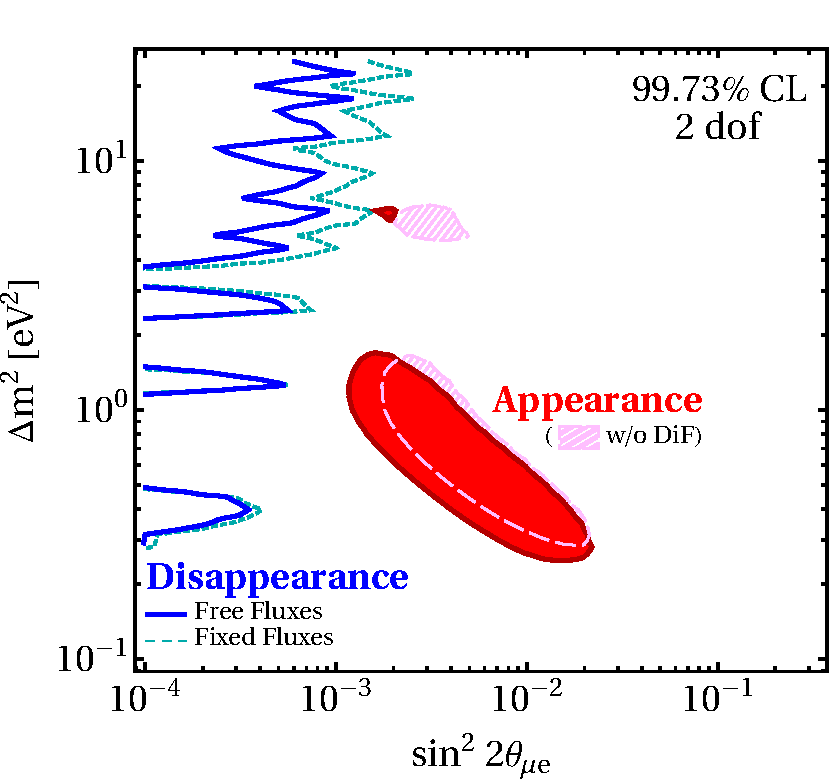
\includegraphics[width=0.7\linewidth]{figures/theory/app-disapp.pdf}
    \caption{Contours delimiting the 99.73\% C.L. ($3\sigma$) regions in mass splitting and the effective mixing angle $\sin^2(2\theta_{\nu e})\equiv 4\abs{U_{\mu 4}}^2\abs{U_{e4}}^2$ from the appearance ($\nu_\mu \rightarrow \nu_e$) channel and the disappearance ($\nu_e \rightarrow \nu_e$) channel. Figure taken from \cite{Dentler_2018}.\label{fig:app-disapp-tension}}
\end{figure}
In order to attribute the observed phenomena to sterile neutrino oscillations, the model would require additional degrees of freedom. One possibility is to give the heavy neutrino state the ability to decay, which can reduce the tension between appearance and disappearance results to the level of $3.2\sigma$\cite{Diaz_2020}. A detailed discussion on global fits of the neutrino anomalies can be found in \sidecite{Diaz_2020}.

\subsection{Other constraints on sterile neutrinos}
While the neutrino oscillation anomalies described in \refsec{global-anomalies} hint at the possibility of an additional neutrino mass eigenstate with a mass splitting o $\Delta m^2_{41} \gtrsim \order{\SI{1}{eV^2}}$, there are other constraints on the masses and number of neutrino flavor states that need to be considered.

\subsubsection{Unitarity constraints on the PNMS matrix}
If the neutrino mixing matrix is extended by adding mass eigenstates, the $3\times3$ block matrix for the three active neutrino flavors is no longer unitary. Therefore, such extensions can be constrained in a generic way by testing the unitarity of the PNMS matrix. Unitarity of the mixing matrix imposes four conditions on the elements of the matrix:
\begin{align}
    |U^{3\nu}_{\alpha 1}|^2 + |U^{3\nu}_{\alpha 2}|^2 + |U^{3\nu}_{\alpha 3}|^2 - 1 = \delta_\alpha &= 0,~~\alpha=e,\mu,\tau, \label{eq:unitarity_1}
    \\
    |U^{3\nu}_{e i}|^2 + |U^{3\nu}_{\mu i}|^2 + |U^{3\nu}_{\tau i}|^2 -1 = \delta_i &= 0,~~i=1,2,3, \label{eq:unitarity_2}
    \\
    U^{3\nu}_{\alpha 1}U^{3\nu,*}_{\beta 1} + U^{3\nu}_{\alpha 2}U^{3\nu,*}_{\beta 2} + U^{3\nu}_{\alpha 3}U^{3\nu,*}_{\beta 3} = \zeta_{\alpha\beta} &= 0,~~\alpha, \beta = e,\mu,\tau,~~\alpha\neq\beta, \label{eq:unitarity_3}
    \\
    U^{3\nu}_{e i}U^{3\nu,*}_{e j} + U^{3\nu}_{\mu i}U^{3\nu,*}_{\mu j} + U^{3\nu}_{\tau i}U^{3\nu,*}_{\tau j} = \zeta_{ij} &= 0,~~i,j  =1,2,3,~~i\neq j. \label{eq:unitarity_4}
\end{align}
The first two conditions in \cref{eq:unitarity_1,eq:unitarity_2} are the normalization of the rows and columns. The third and fourth conditions in \cref{eq:unitarity_3,eq:unitarity_4} are the triangle closure conditions. A global analysis constraining the degree to which each of these conditions can be violated given the experimental data can be found in \sidecite{global_unitarity_Hu}. The analysis in \cite{global_unitarity_Hu} combines non-anomalous measurements from reactor, solar, and long-baseline accelerator experiments as well as several published sterile neutrino searches. The reactor data used is exclusively comprised of those experiments that have a near and far detector setup and constraints are derived using only ratios between fluxes at different baselines. The accelerator data consists of non-anomalous measurements from NO$\nu$A and T2K. The $\chi^2$ test statistic for the quantities in \crefrange{eq:unitarity_1}{eq:unitarity_4} calculated in \cite{global_unitarity_Hu} are shown in \reffig{nonunitary-global-fits}. No evidence for non-unitarity is found. The normalization of the $|U_{ei}|$ row is constrained to $\order{\num{e-3}}$, which puts the result in strong tension with the sterile neutrino interpretation of the Gallium anomaly.
\begin{figure}
    \centering
    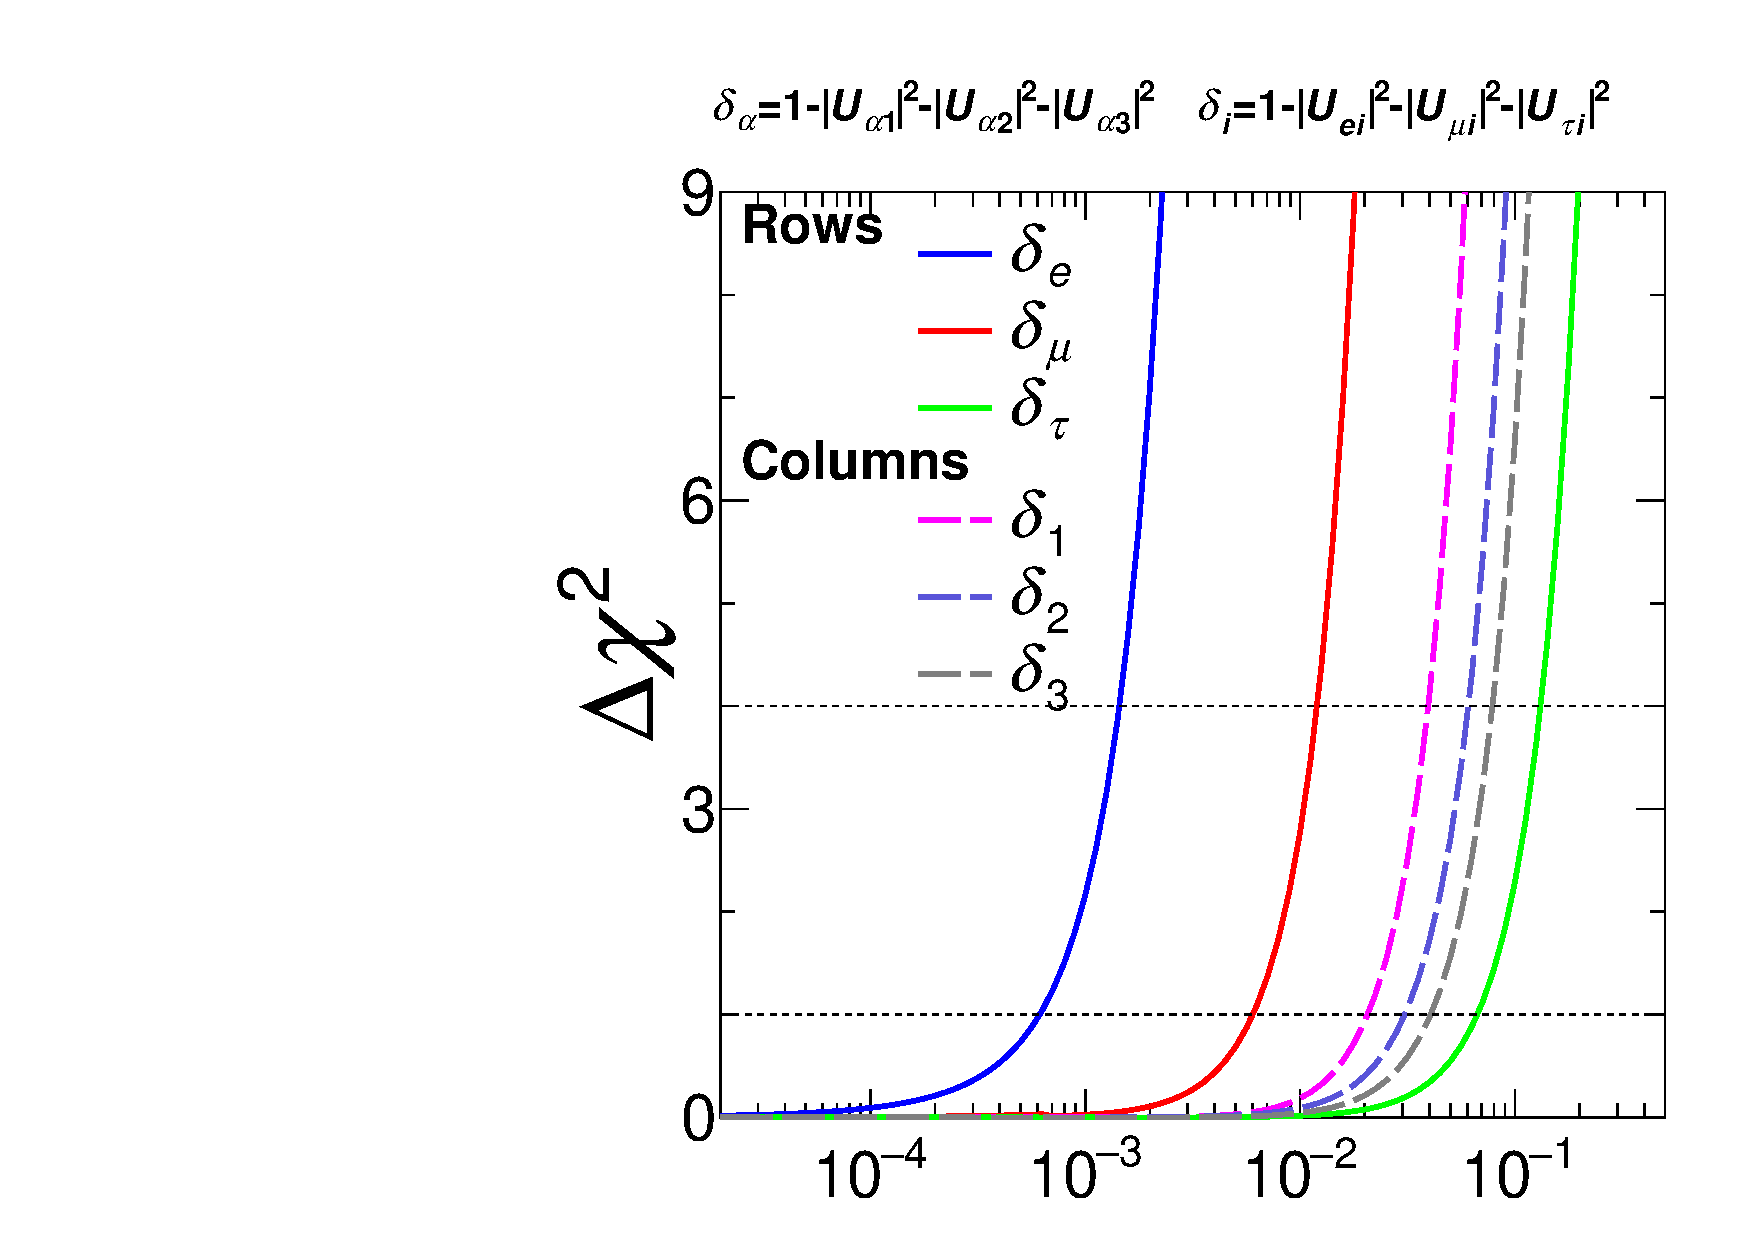
\includegraphics[width=0.49\linewidth]{figures/theory/Norm.pdf}
    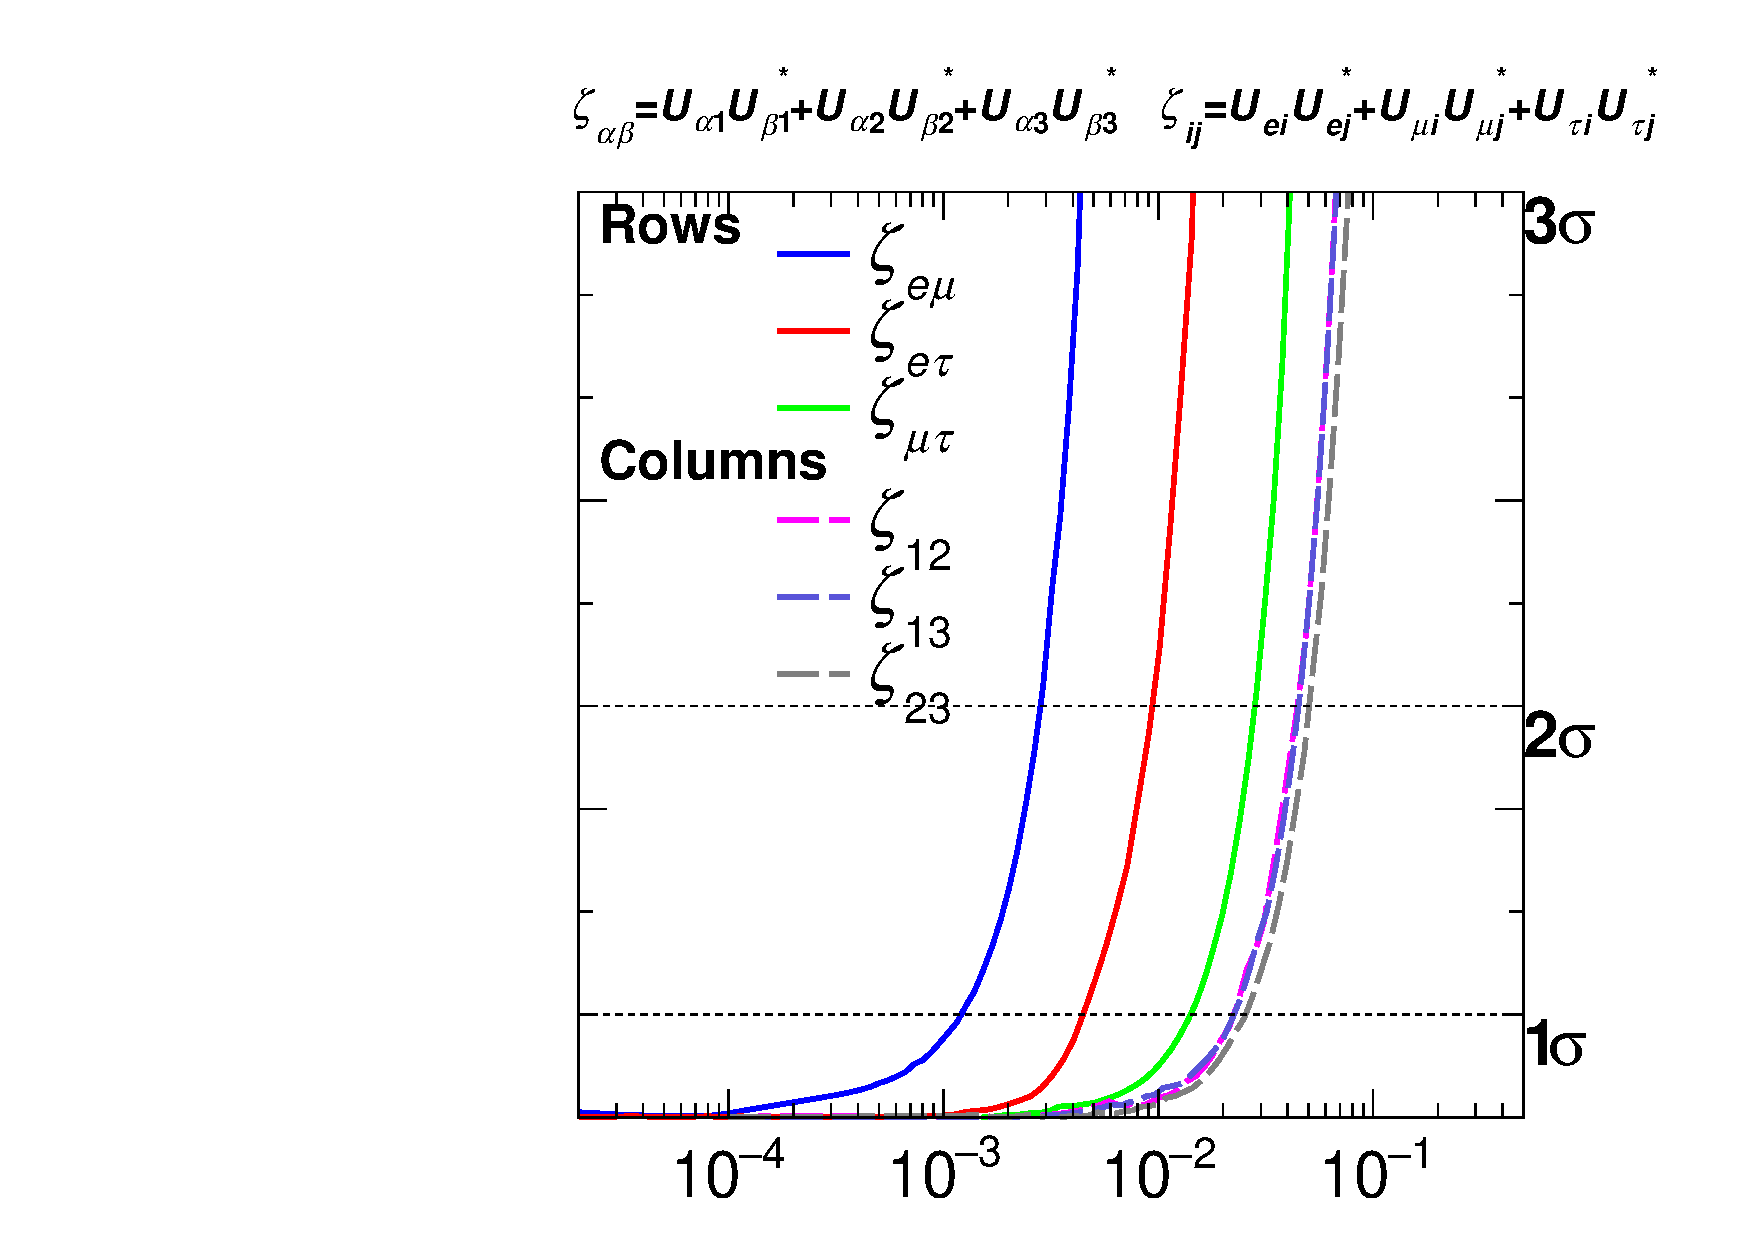
\includegraphics[width=0.49\linewidth]{figures/theory/Clos_temp.pdf}
    \caption{Test statistic for the magnitudes of unitary condition violations calculated in \cite{global_unitarity_Hu}. The shown quantities correspond to those in \crefrange{eq:unitarity_1}{eq:unitarity_4}.\label{fig:nonunitary-global-fits}}
\end{figure}

\subsubsection{Cosmological constraints}
Standard model cosmology places constraints on the number of relativistic neutrino species, $N_\mathrm{eff}$, and the sum of neutrino masses, $\sum m_\nu$. Both of these parameters can be estimated from observations of the cosmic microwave background (CMB), the large scale structures, and the abundance of light elements from Big Bang Nucleosynthesis. Recent results from the Planck collaboration for these parameters are $N_\mathrm{eff}=\num{2.99+-0.17}$ and $\sum m_\nu < \SI{0.1}{eV}$\sidecite{Planck2018}. These results are compatible with the absence of additional heavy neutrino states and are in severe tension with hypotheses involving a mass eigenstate with $\Delta m^2_{41} \sim \order{\SI{1}{eV}}$. This tension can only be alleviated by the introduction of further extensions to the standard model.
